% Upload selected assets to the Overleaf project root.
\begin{figure}[htbp]\centering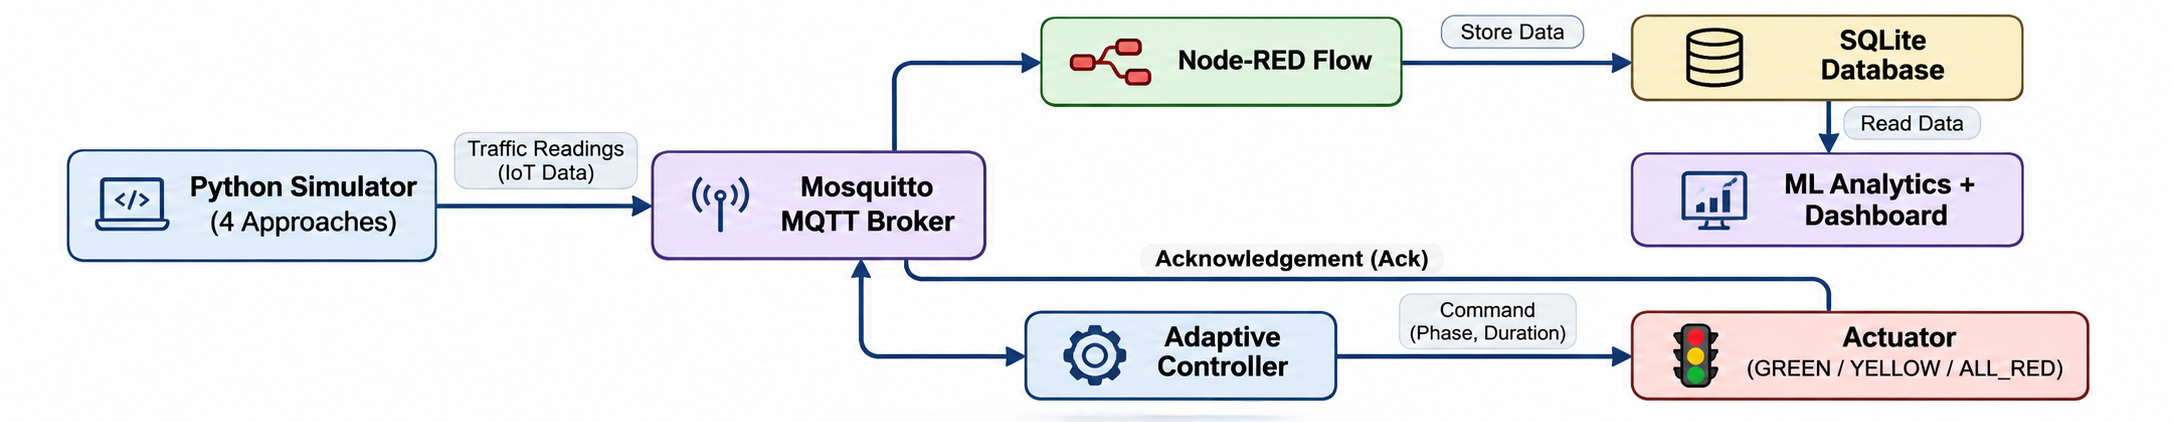
\includegraphics[width=.95\textwidth]{report_assets/fig_architecture.png}\caption{Architecture of the simulated adaptive traffic signal controller.}\label{fig:architecture}\end{figure}
\begin{figure}[htbp]\centering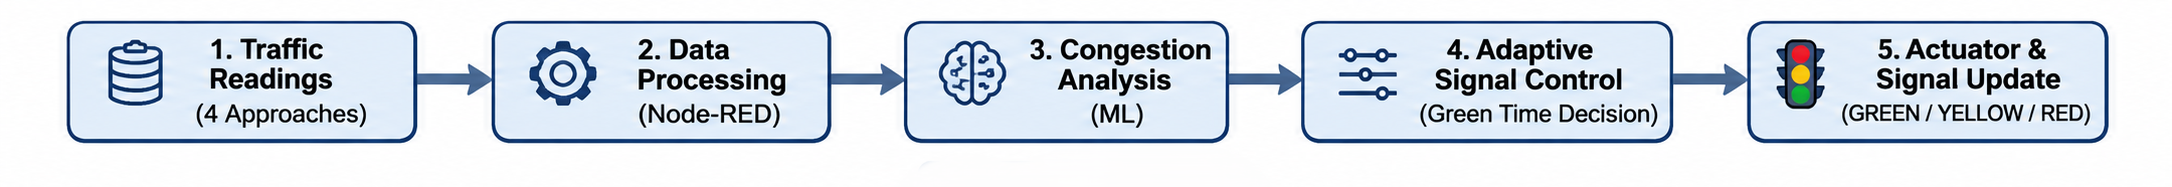
\includegraphics[width=.95\textwidth]{report_assets/fig_workflow.png}\caption{Workflow from readings to rule-based live control and actuator acknowledgement. Update the diagram to show ML separately as offline analysis.}\label{fig:workflow}\end{figure}
\begin{figure}[htbp]\centering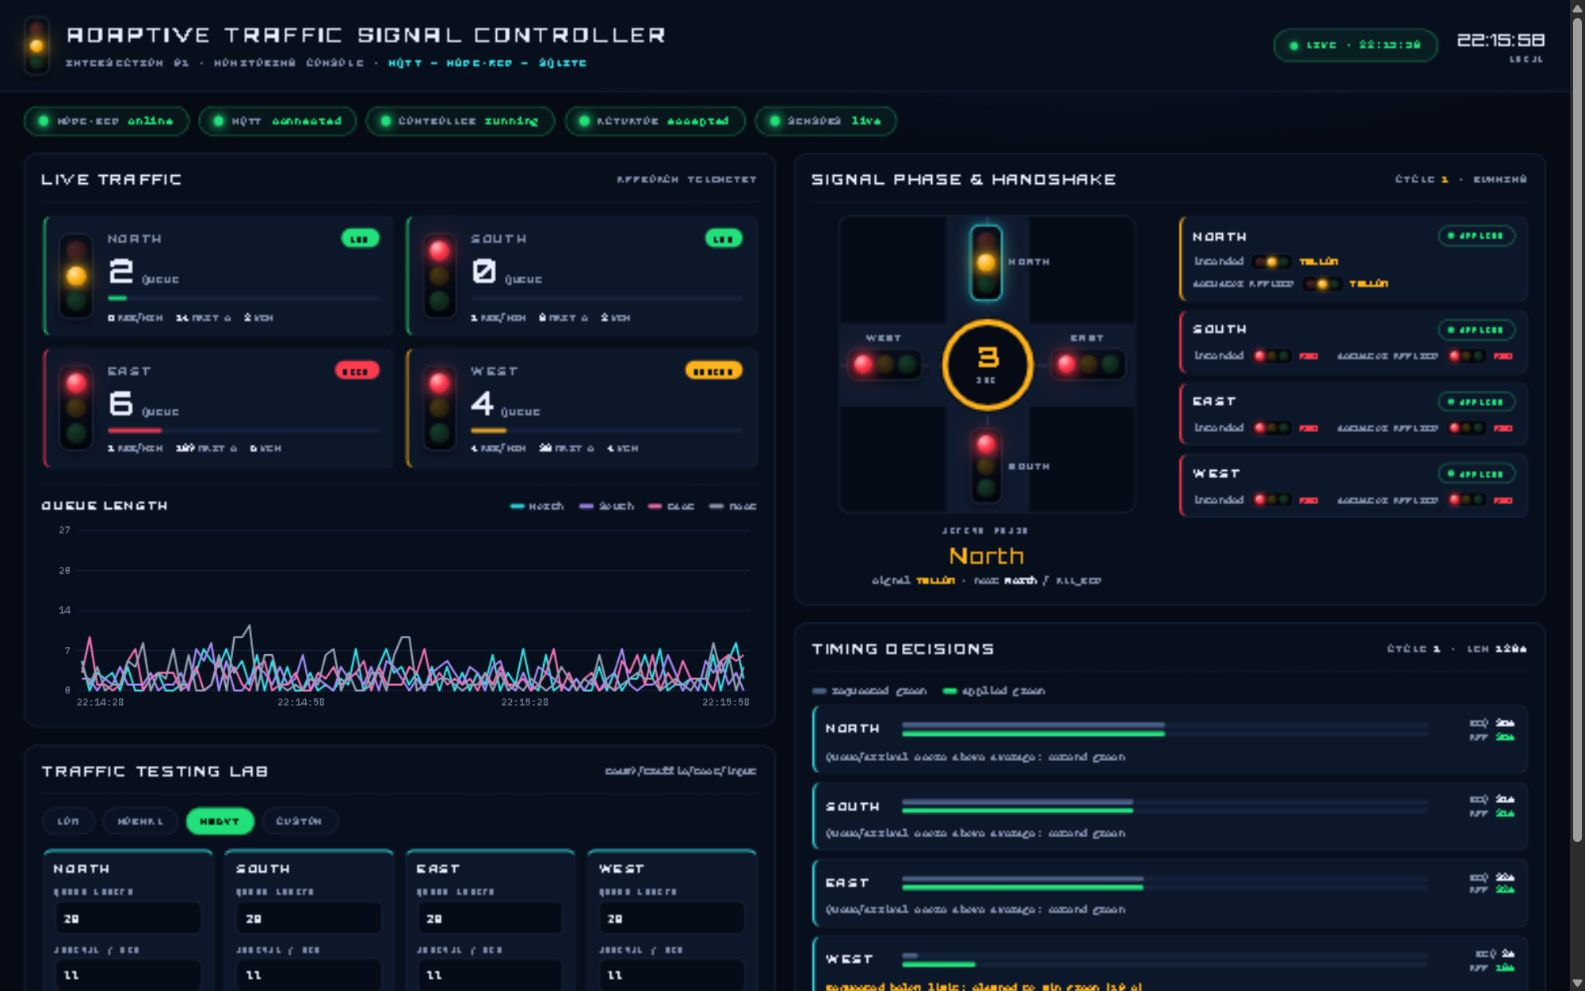
\includegraphics[width=.98\textwidth]{report_assets/dashboard/dashboard_overview.png}\caption{Overview of the running traffic dashboard.}\label{fig:dashboard-overview}\end{figure}
\begin{figure}[htbp]\centering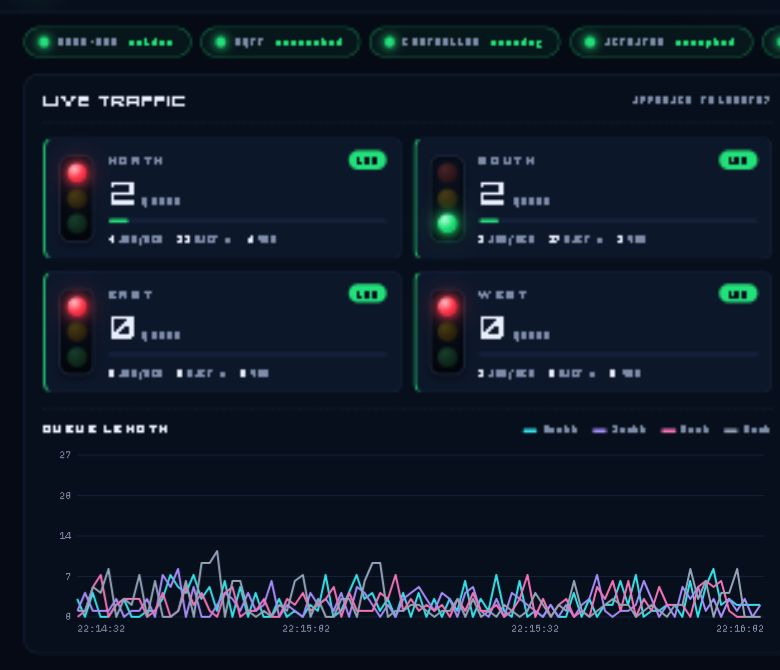
\includegraphics[width=.98\textwidth]{report_assets/dashboard/dashboard_traffic_analytics.png}\caption{Dashboard queue trends and per-approach analytics.}\label{fig:dashboard-analytics}\end{figure}
\begin{figure}[htbp]\centering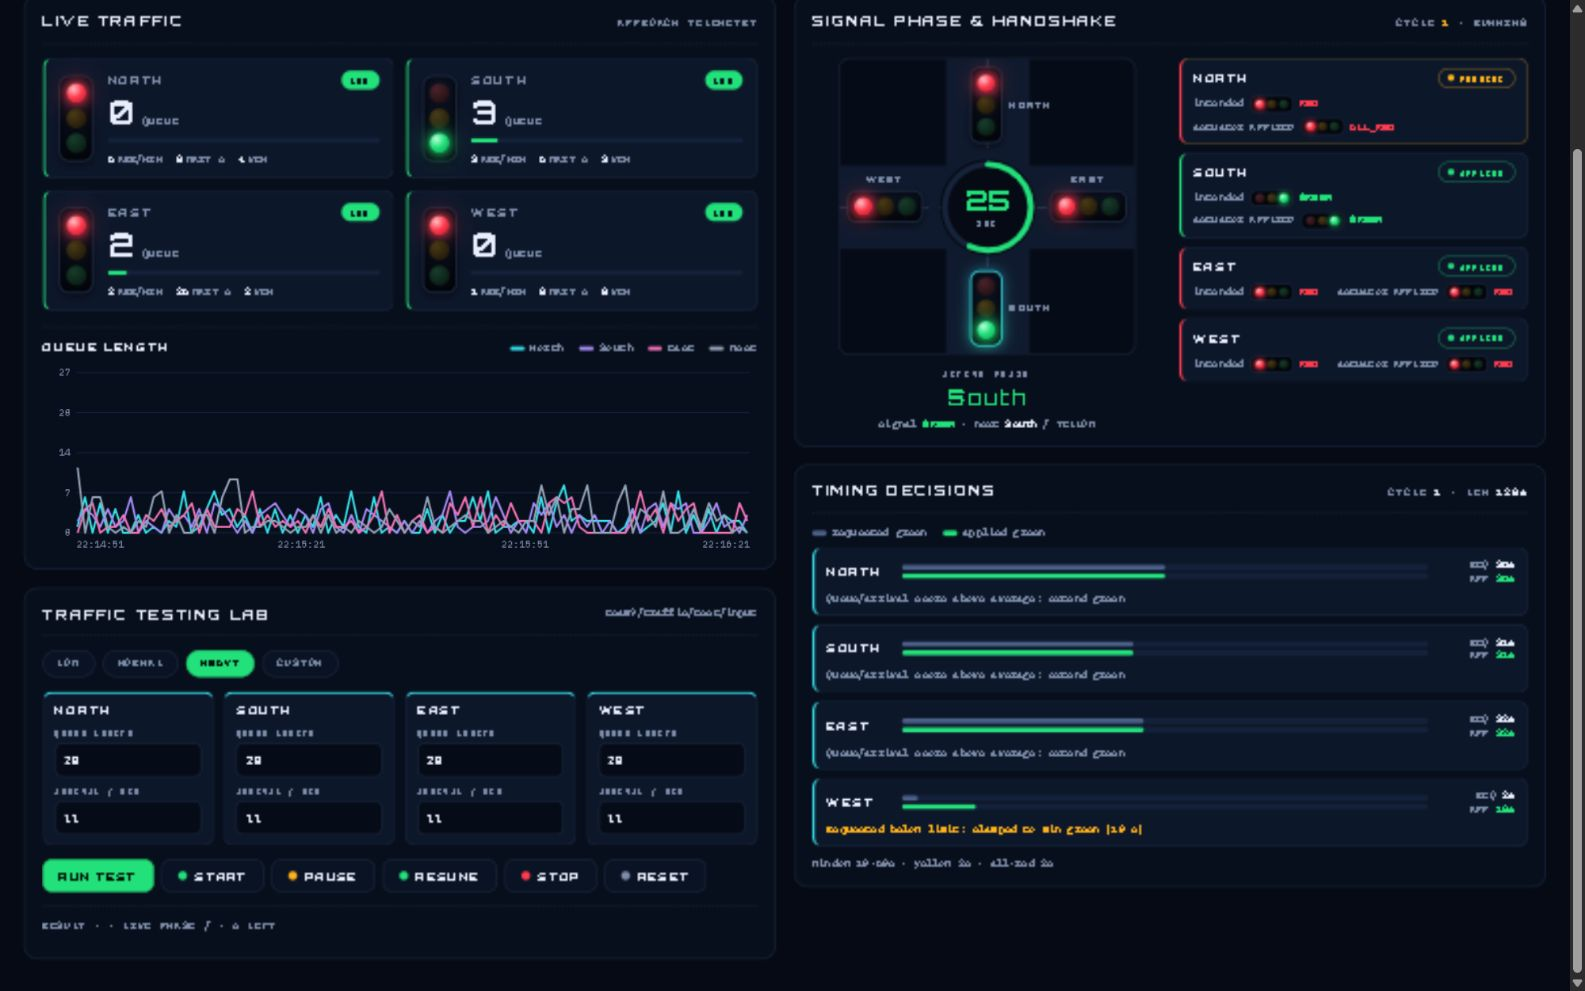
\includegraphics[width=.98\textwidth]{report_assets/dashboard/dashboard_signal_timing.png}\caption{Dashboard timing and signal states.}\label{fig:dashboard-signal-timing}\end{figure}
\begin{figure}[htbp]\centering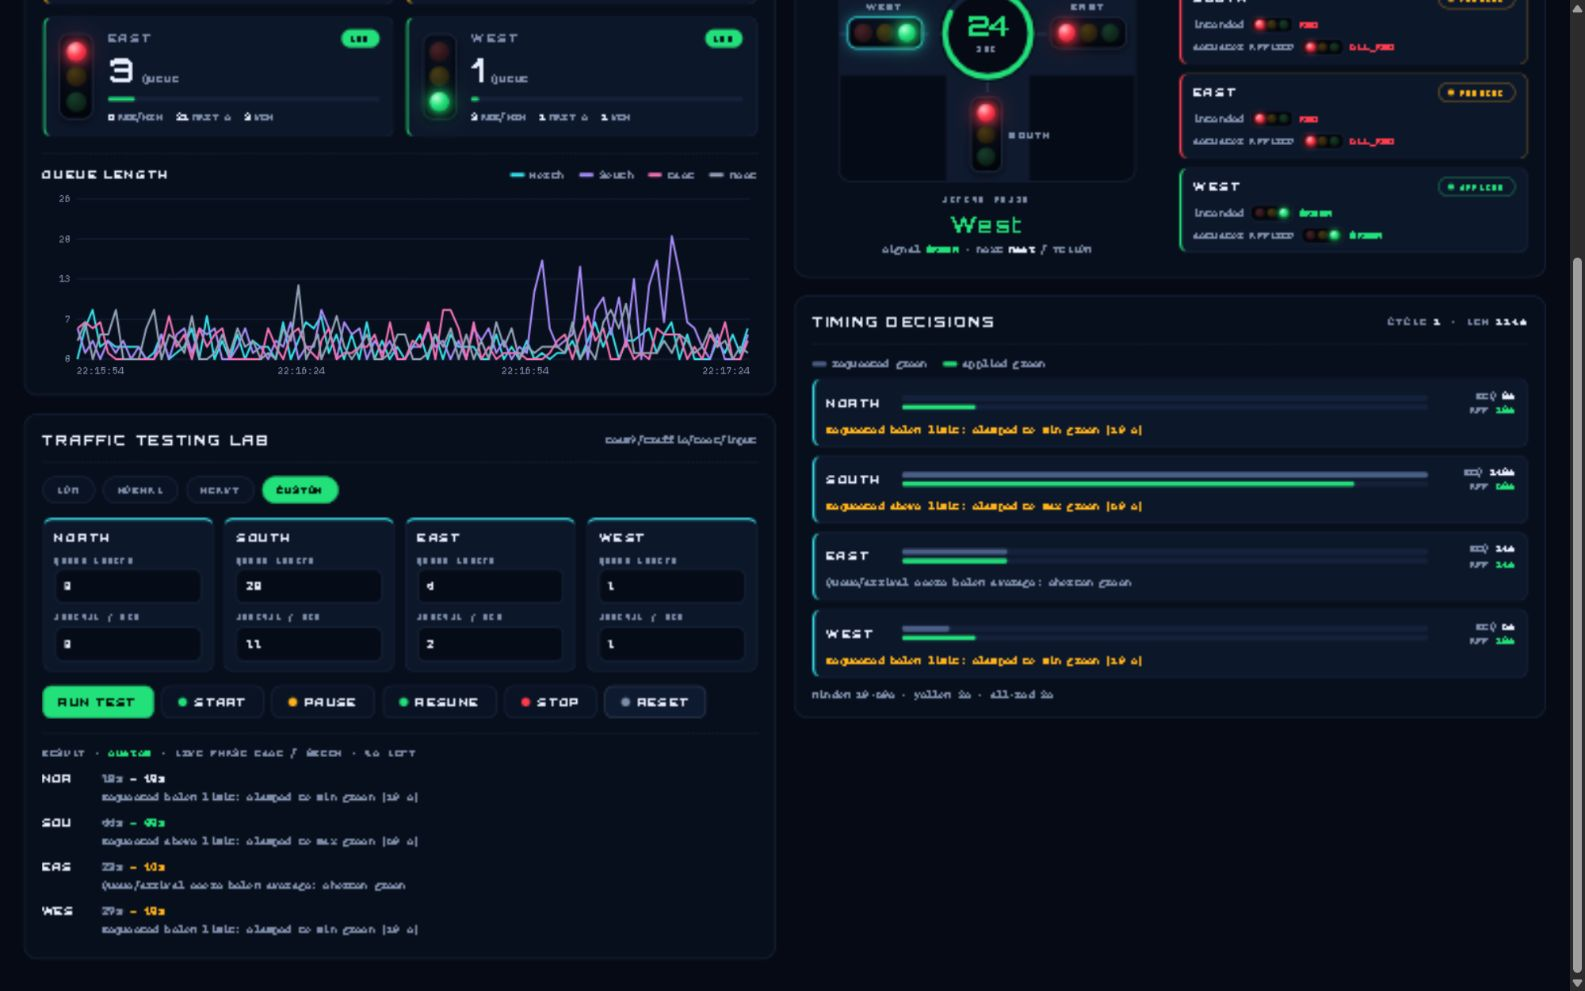
\includegraphics[width=.98\textwidth]{report_assets/dashboard/dashboard_testing_lab.png}\caption{Testing lab scenario and output.}\label{fig:dashboard-lab}\end{figure}
\begin{figure}[htbp]\centering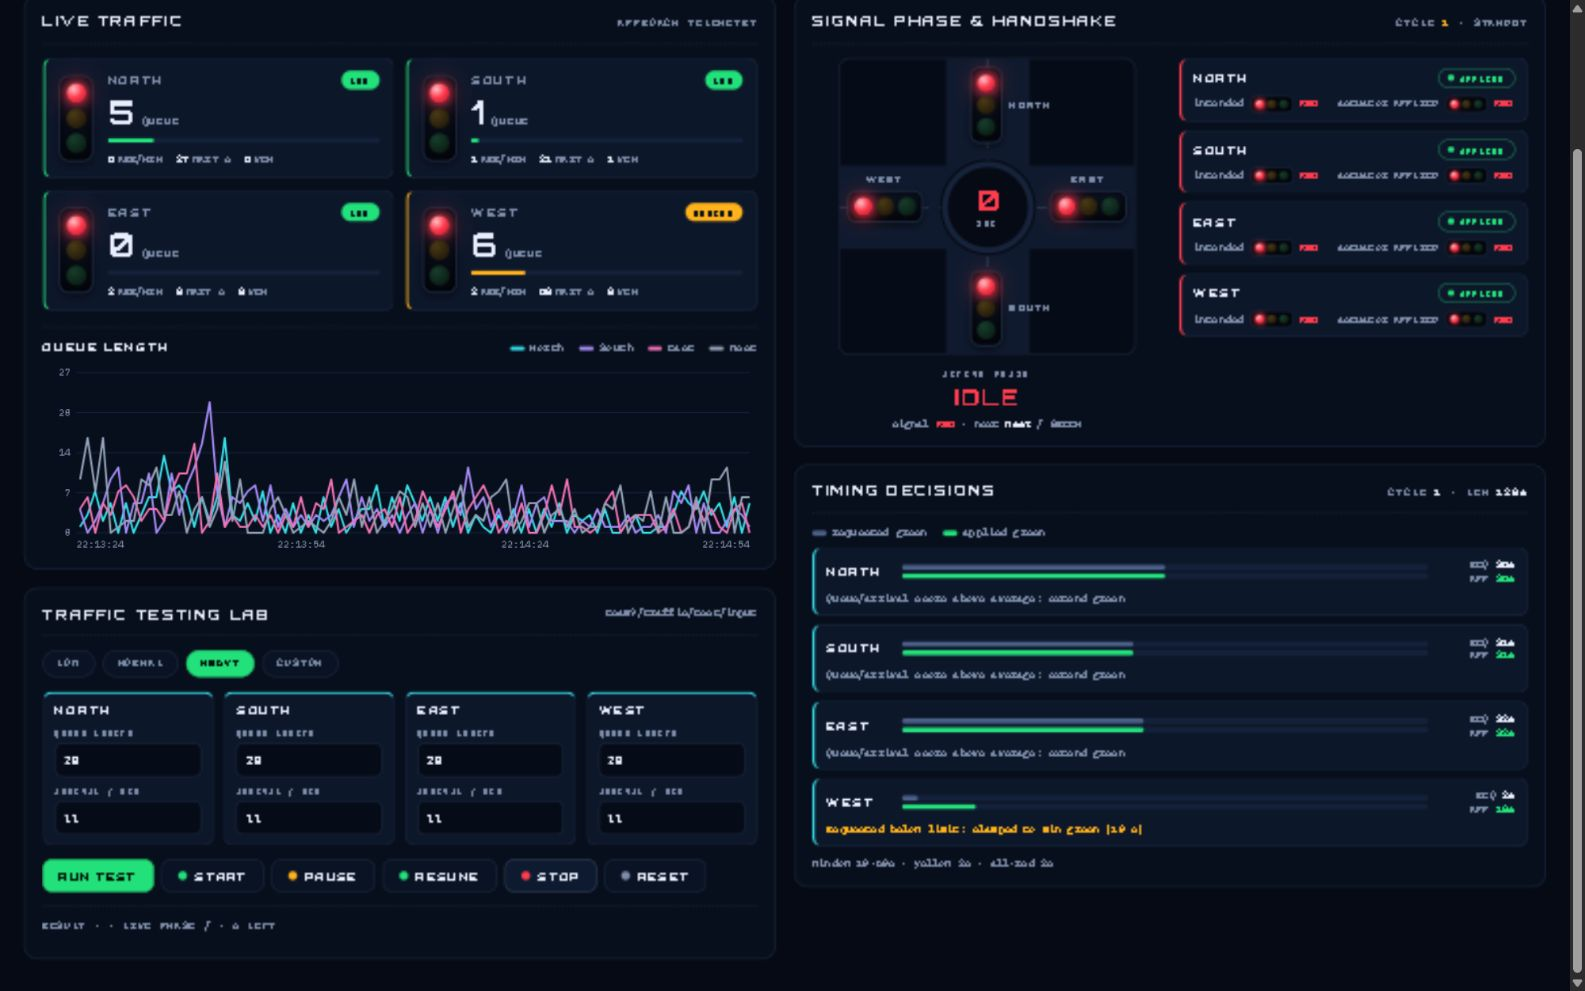
\includegraphics[width=.98\textwidth]{report_assets/dashboard/dashboard_stop_reset_ack.png}\caption{Stop/Reset and actuator-reported RED states; the image does not expose command IDs.}\label{fig:dashboard-stop-reset}\end{figure}
\begin{figure}[htbp]\centering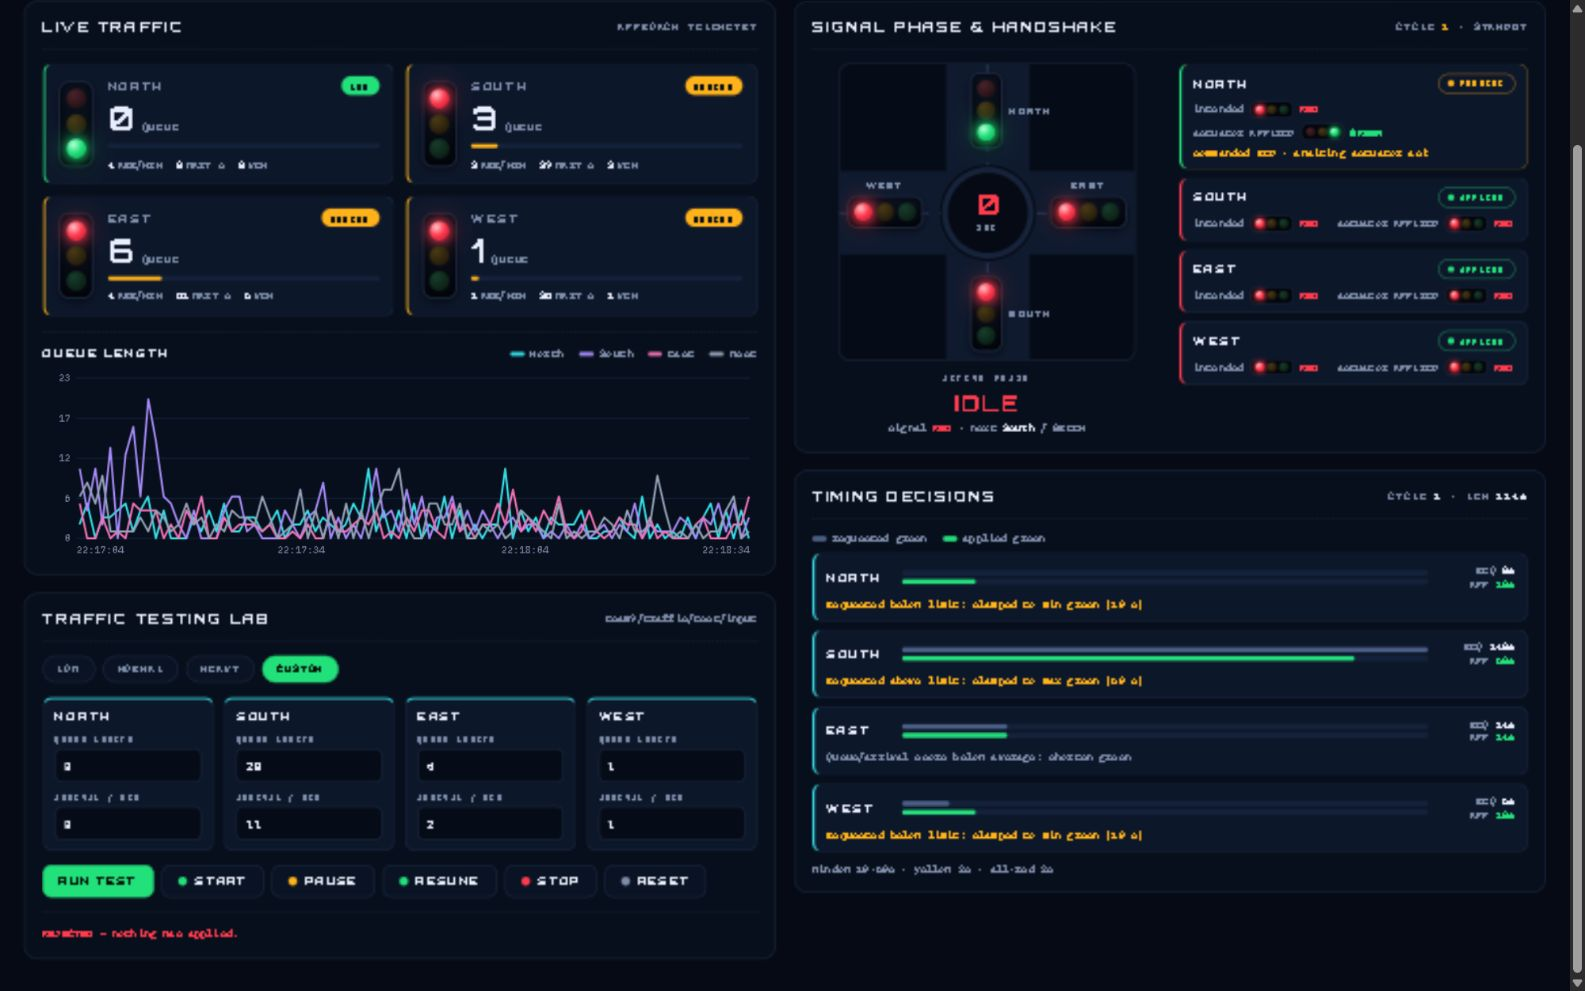
\includegraphics[width=.98\textwidth]{report_assets/dashboard/dashboard_ack_fault_handling.png}\caption{Withheld-ACK test: Stop remains unconfirmed.}\label{fig:dashboard-fault}\end{figure}
\begin{figure}[htbp]\centering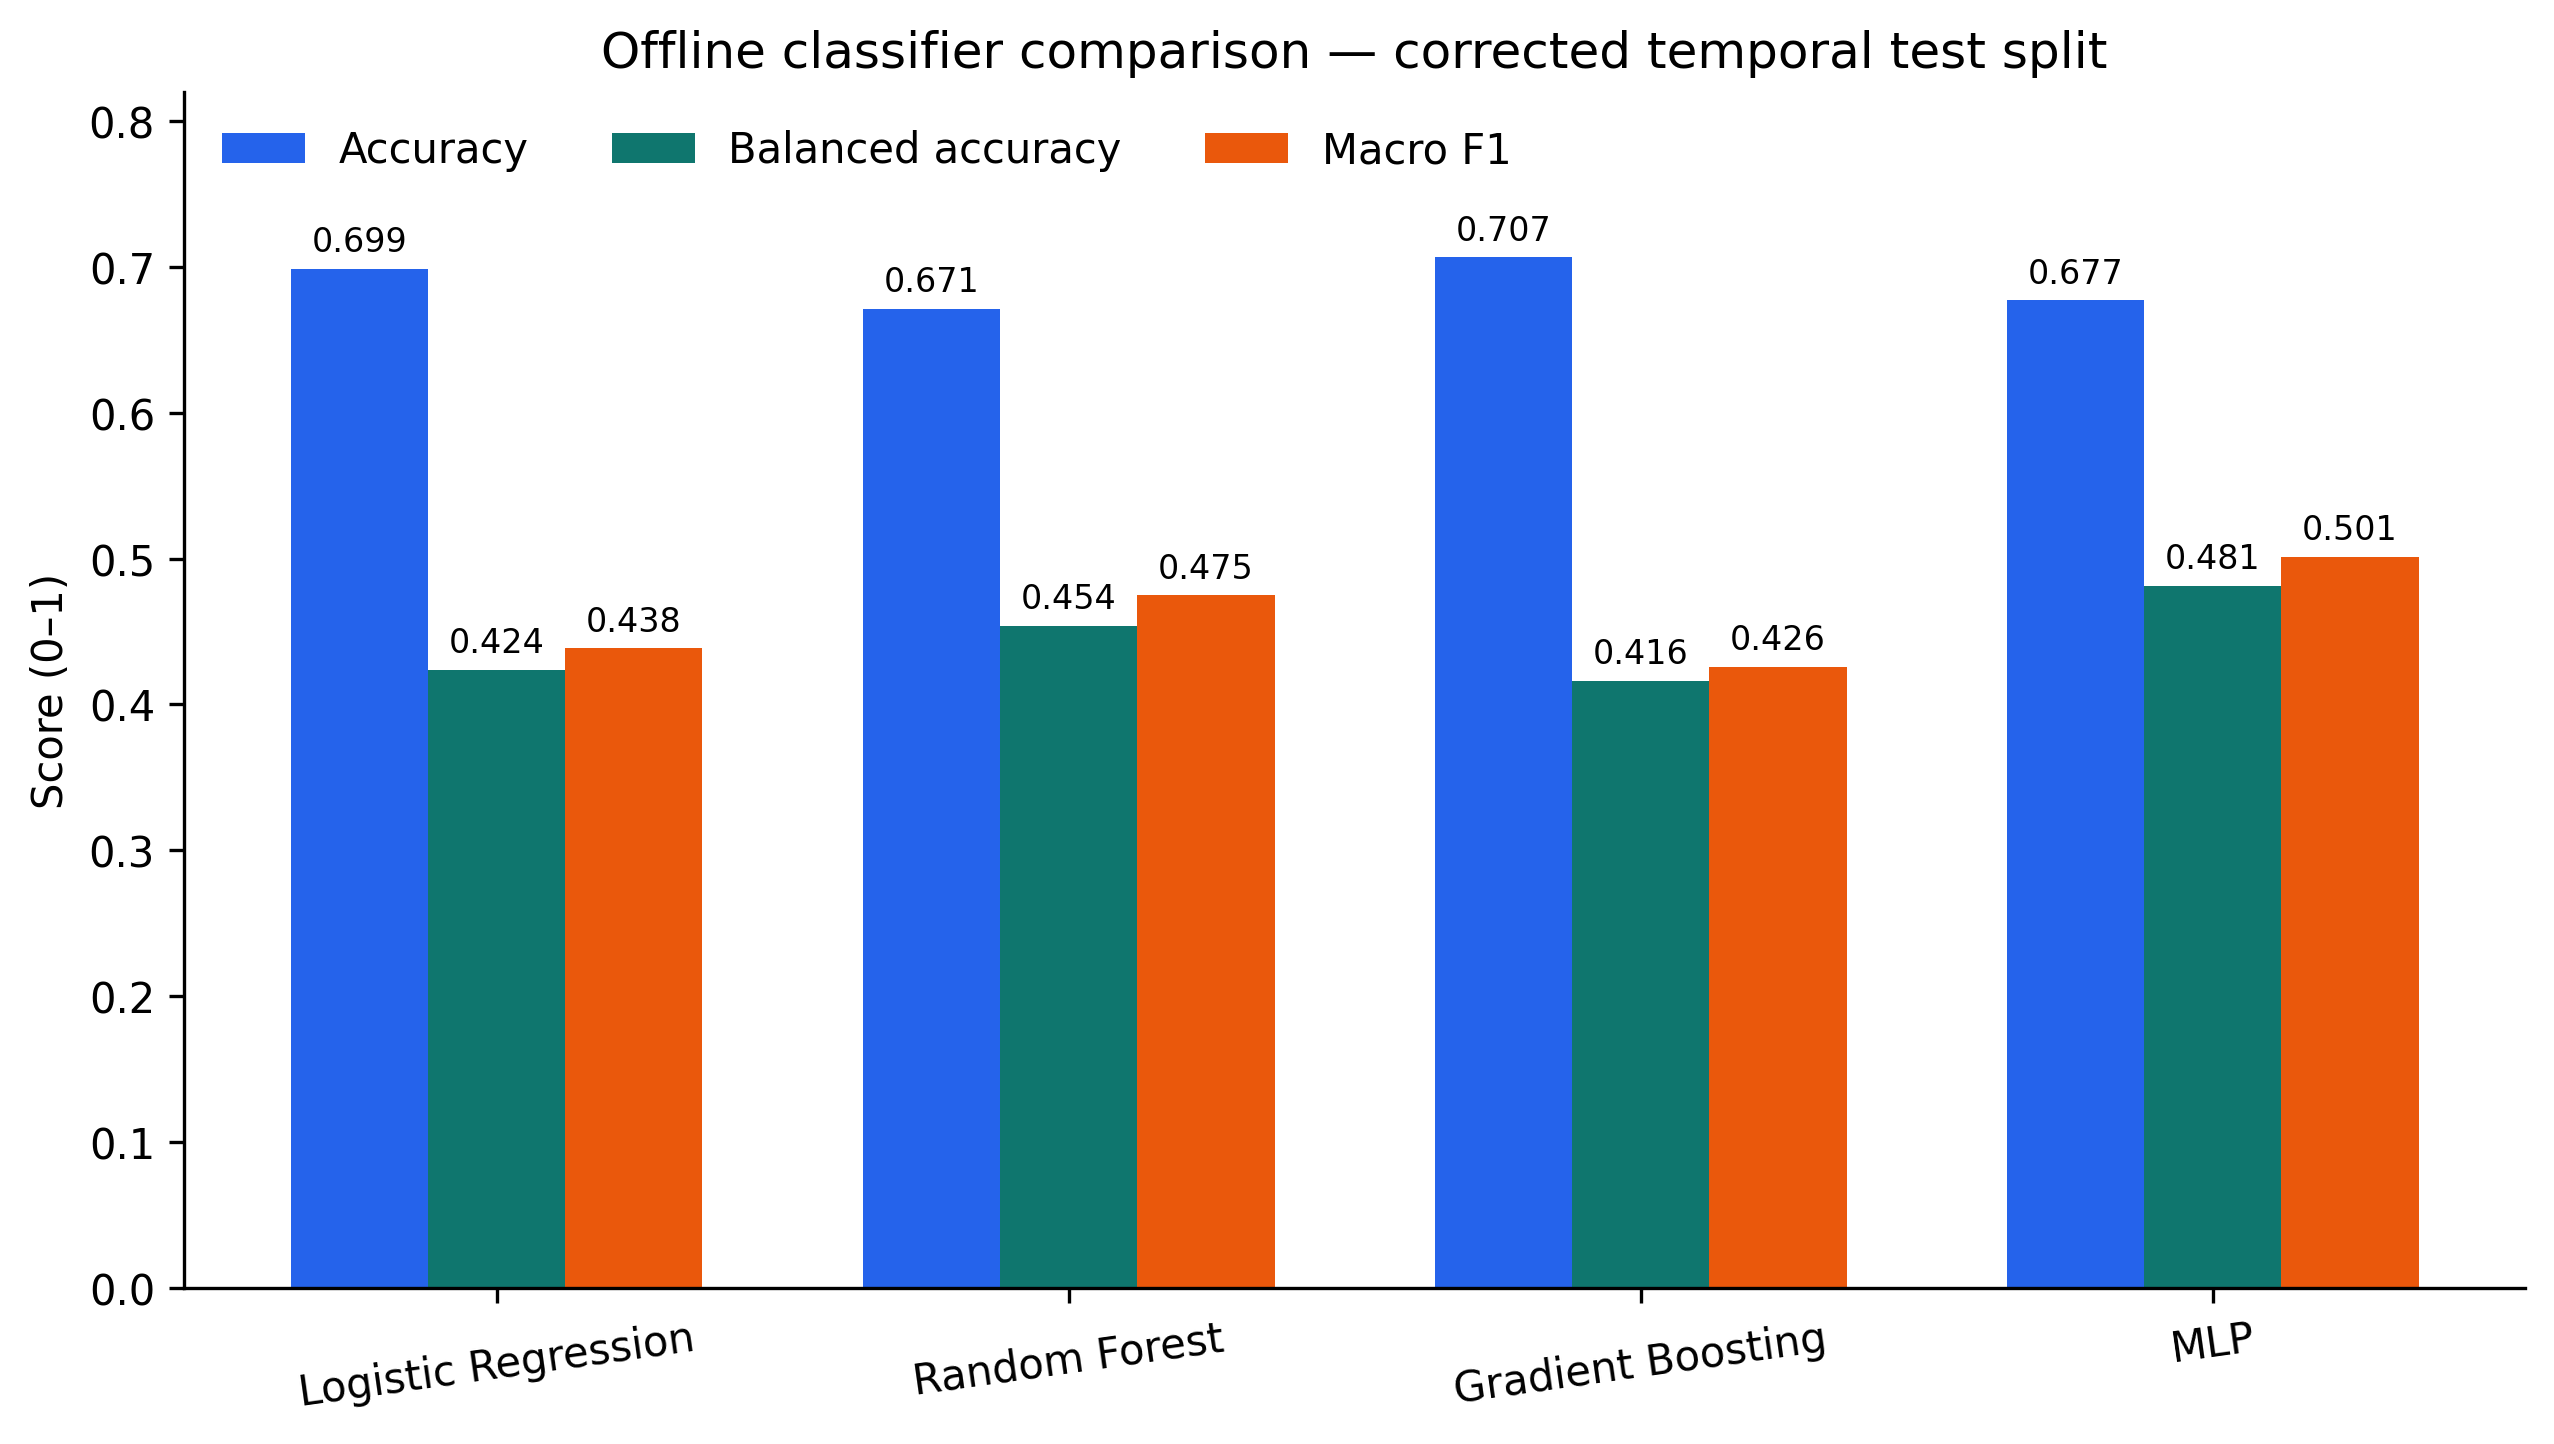
\includegraphics[width=.95\textwidth]{report_assets/graphs/model_comparison_metrics.png}\caption{Four classifiers on the corrected temporal test split.}\label{fig:ml-metrics}\end{figure}
\begin{figure}[htbp]\centering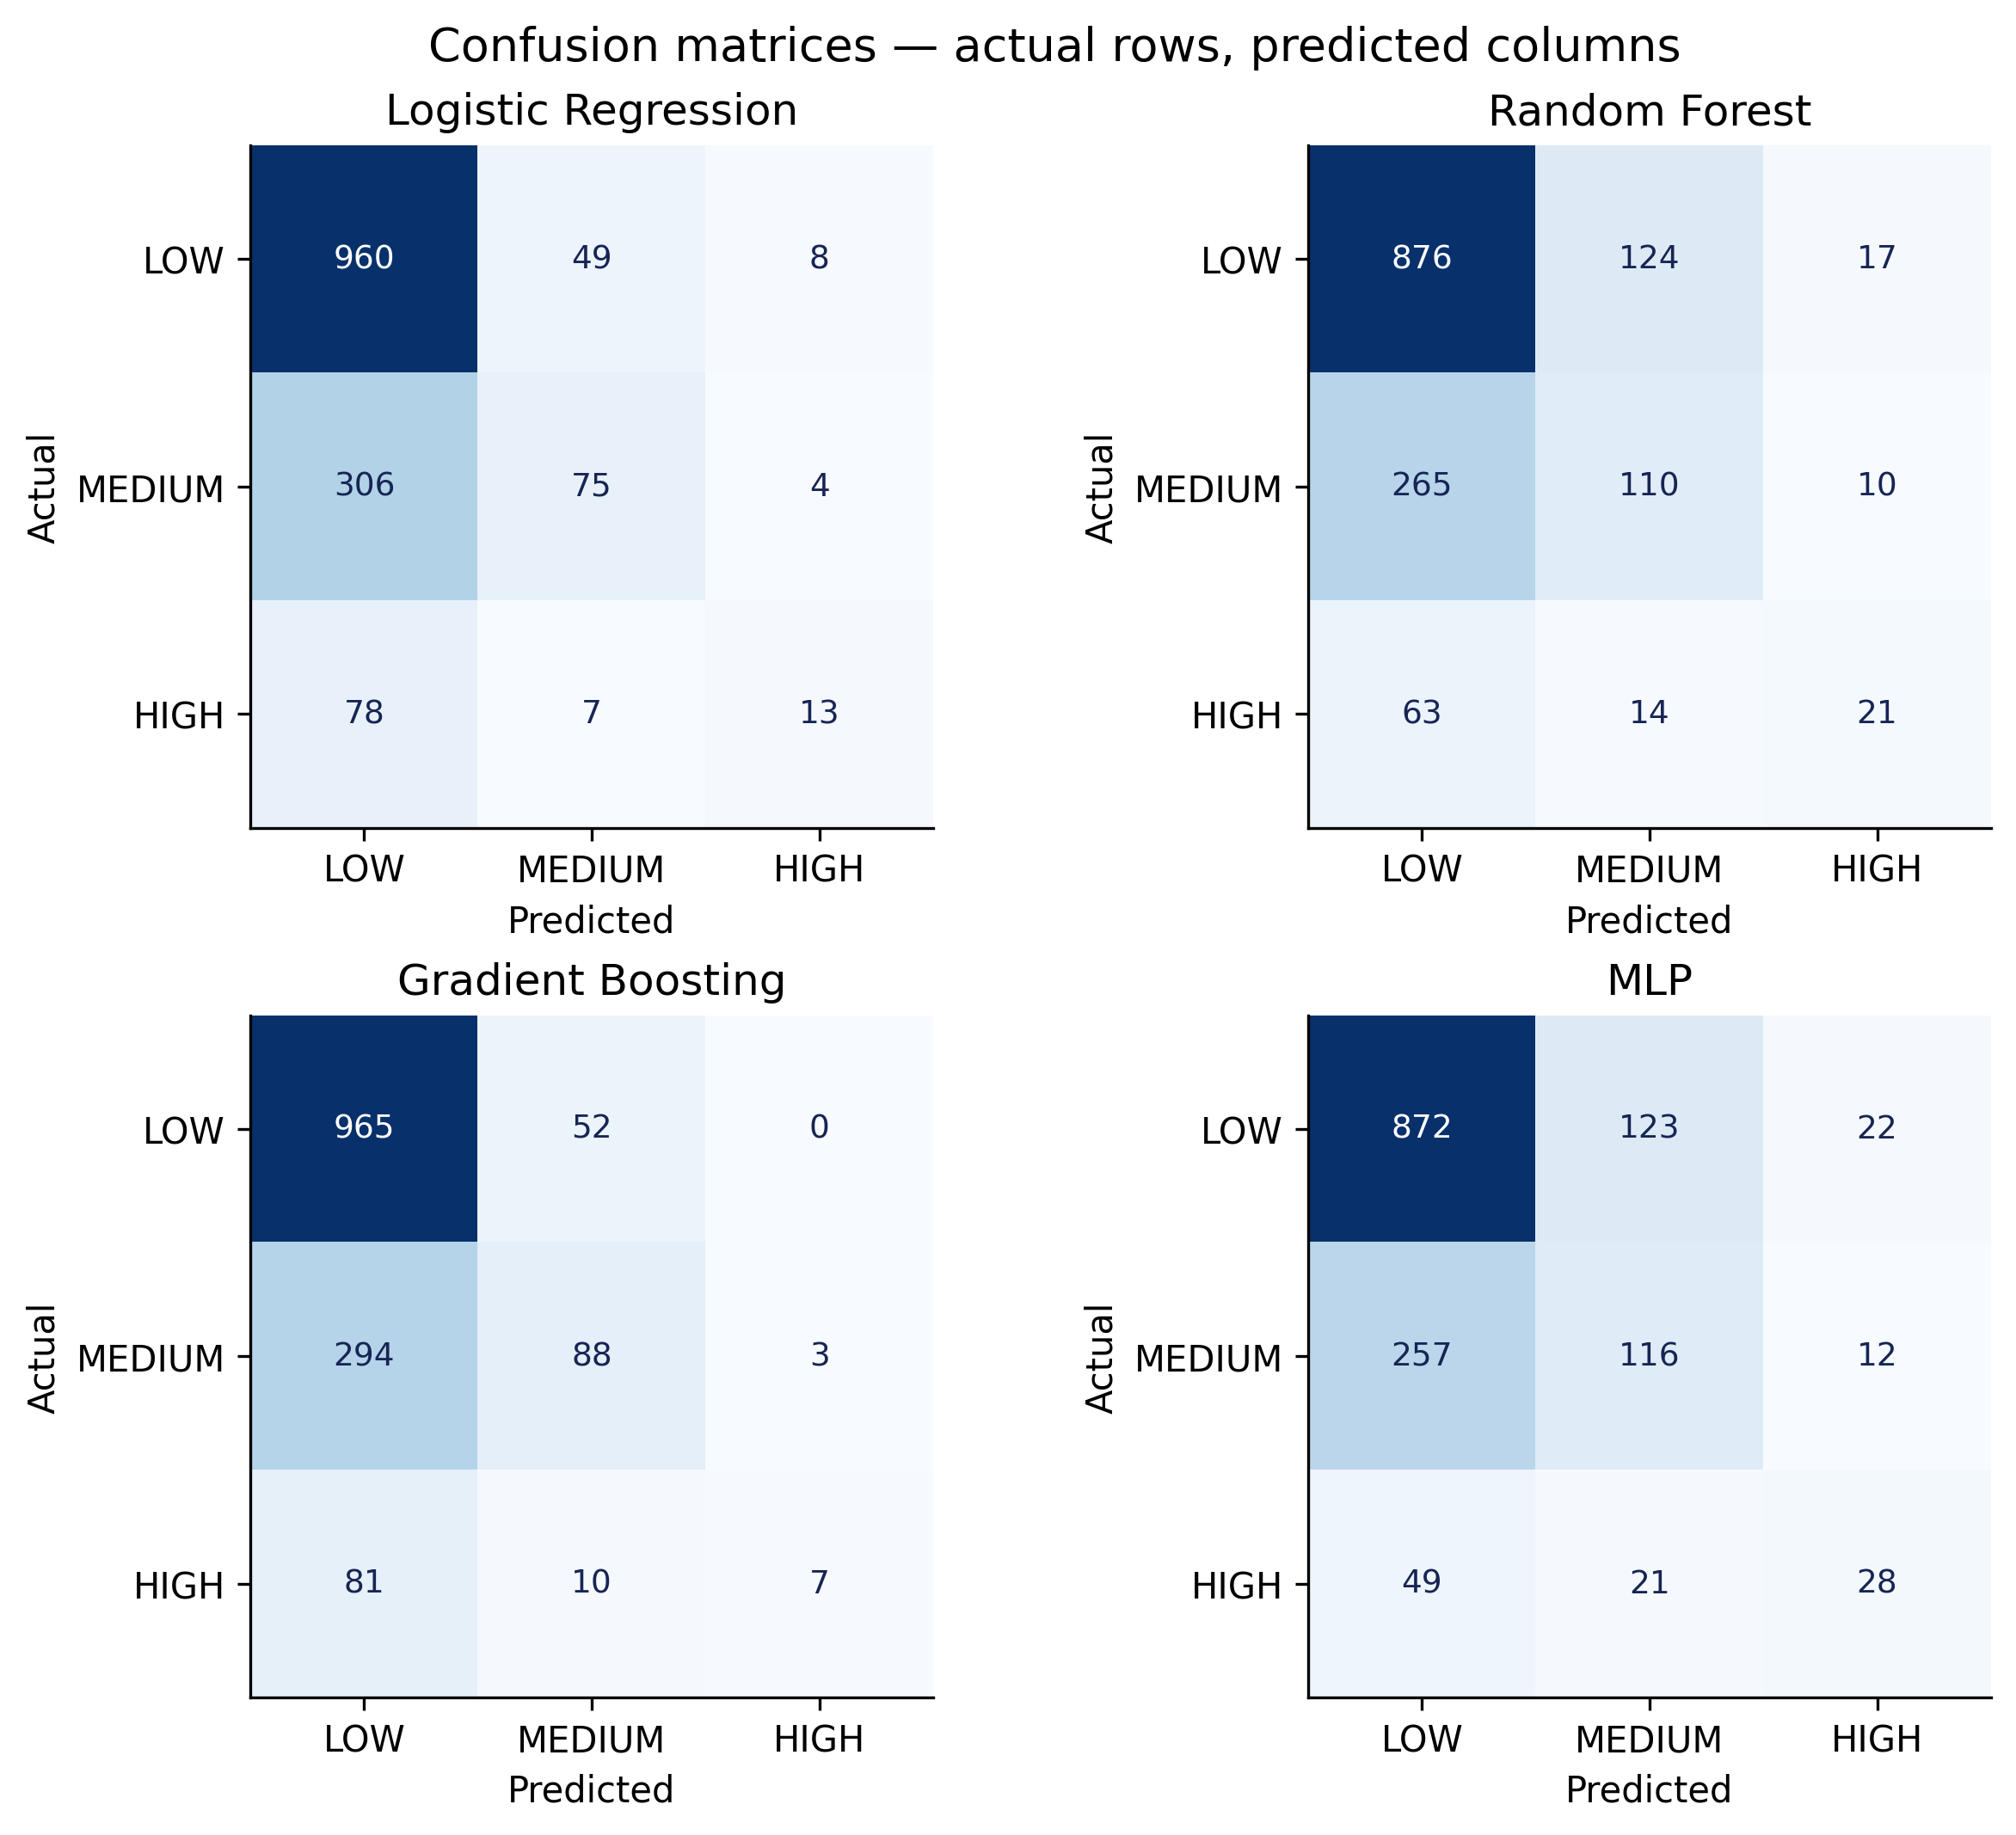
\includegraphics[width=.95\textwidth]{report_assets/graphs/model_comparison_confusion_matrices.png}\caption{Confusion matrices (actual rows, predicted columns) for the corrected temporal test set.}\label{fig:ml-confusion}\end{figure}
\begin{figure}[htbp]\centering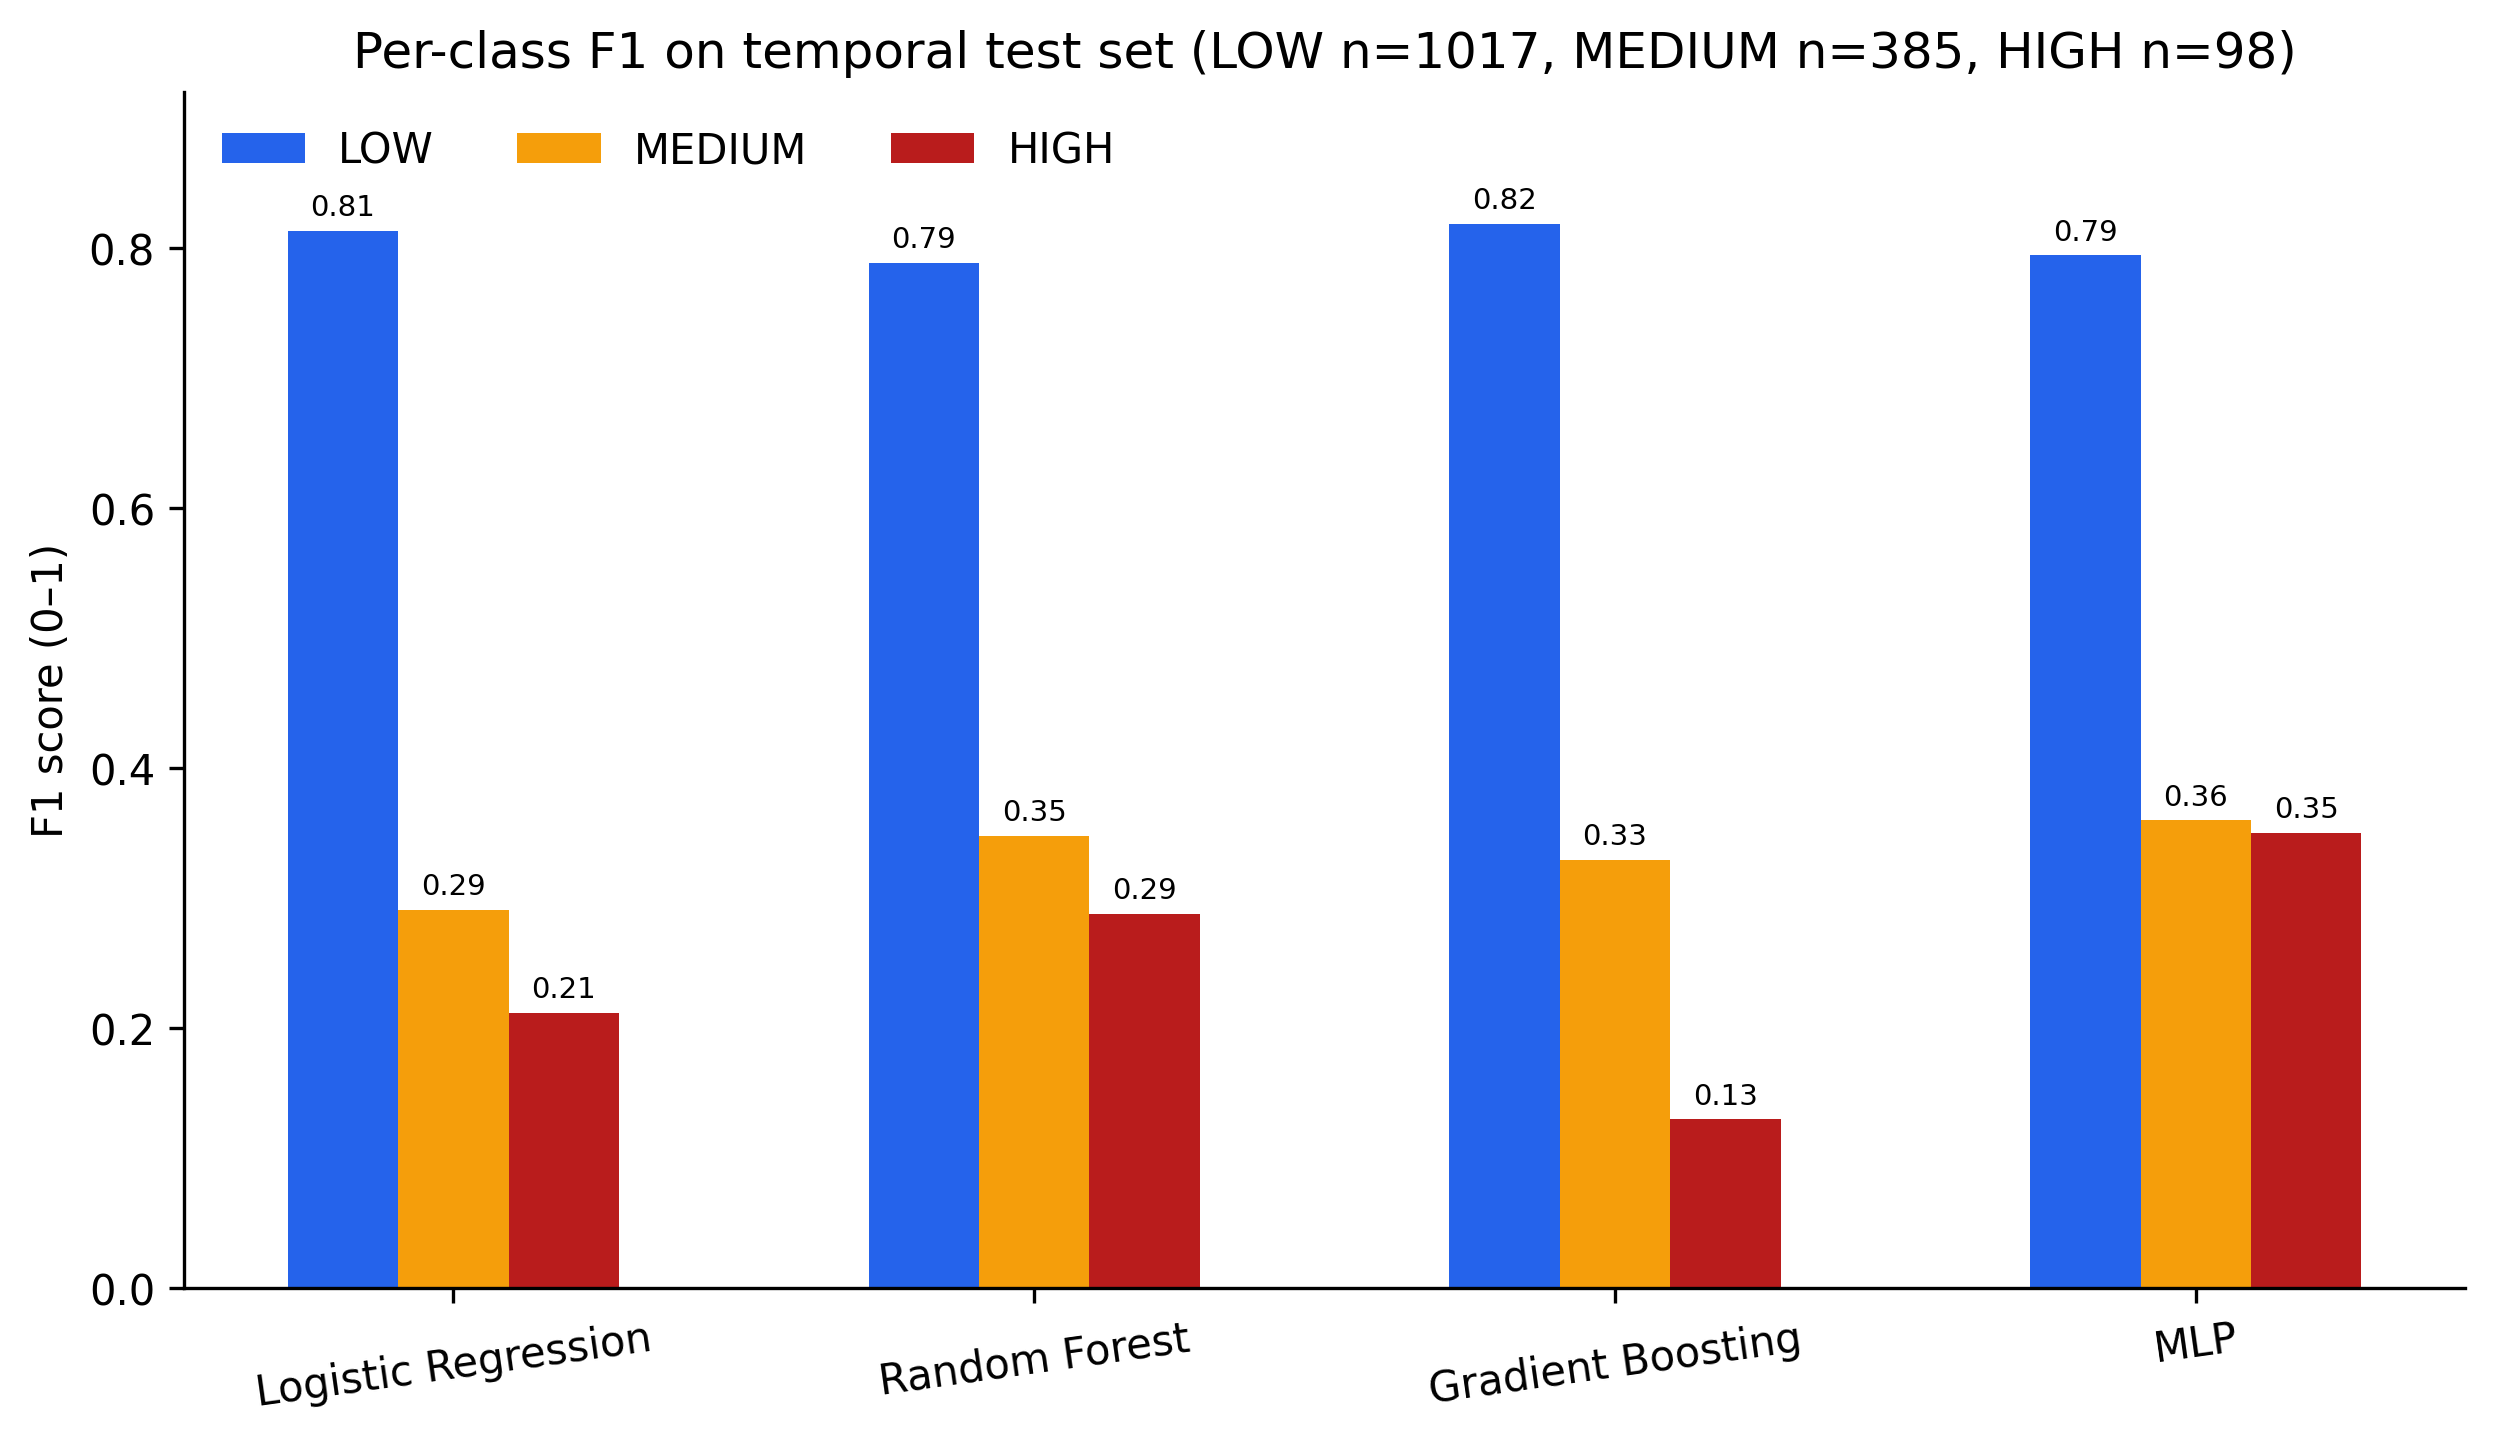
\includegraphics[width=.95\textwidth]{report_assets/graphs/model_comparison_per_class_f1.png}\caption{Per-class F1; HIGH congestion detection remains limited.}\label{fig:ml-per-class}\end{figure}
\begin{figure}[htbp]\centering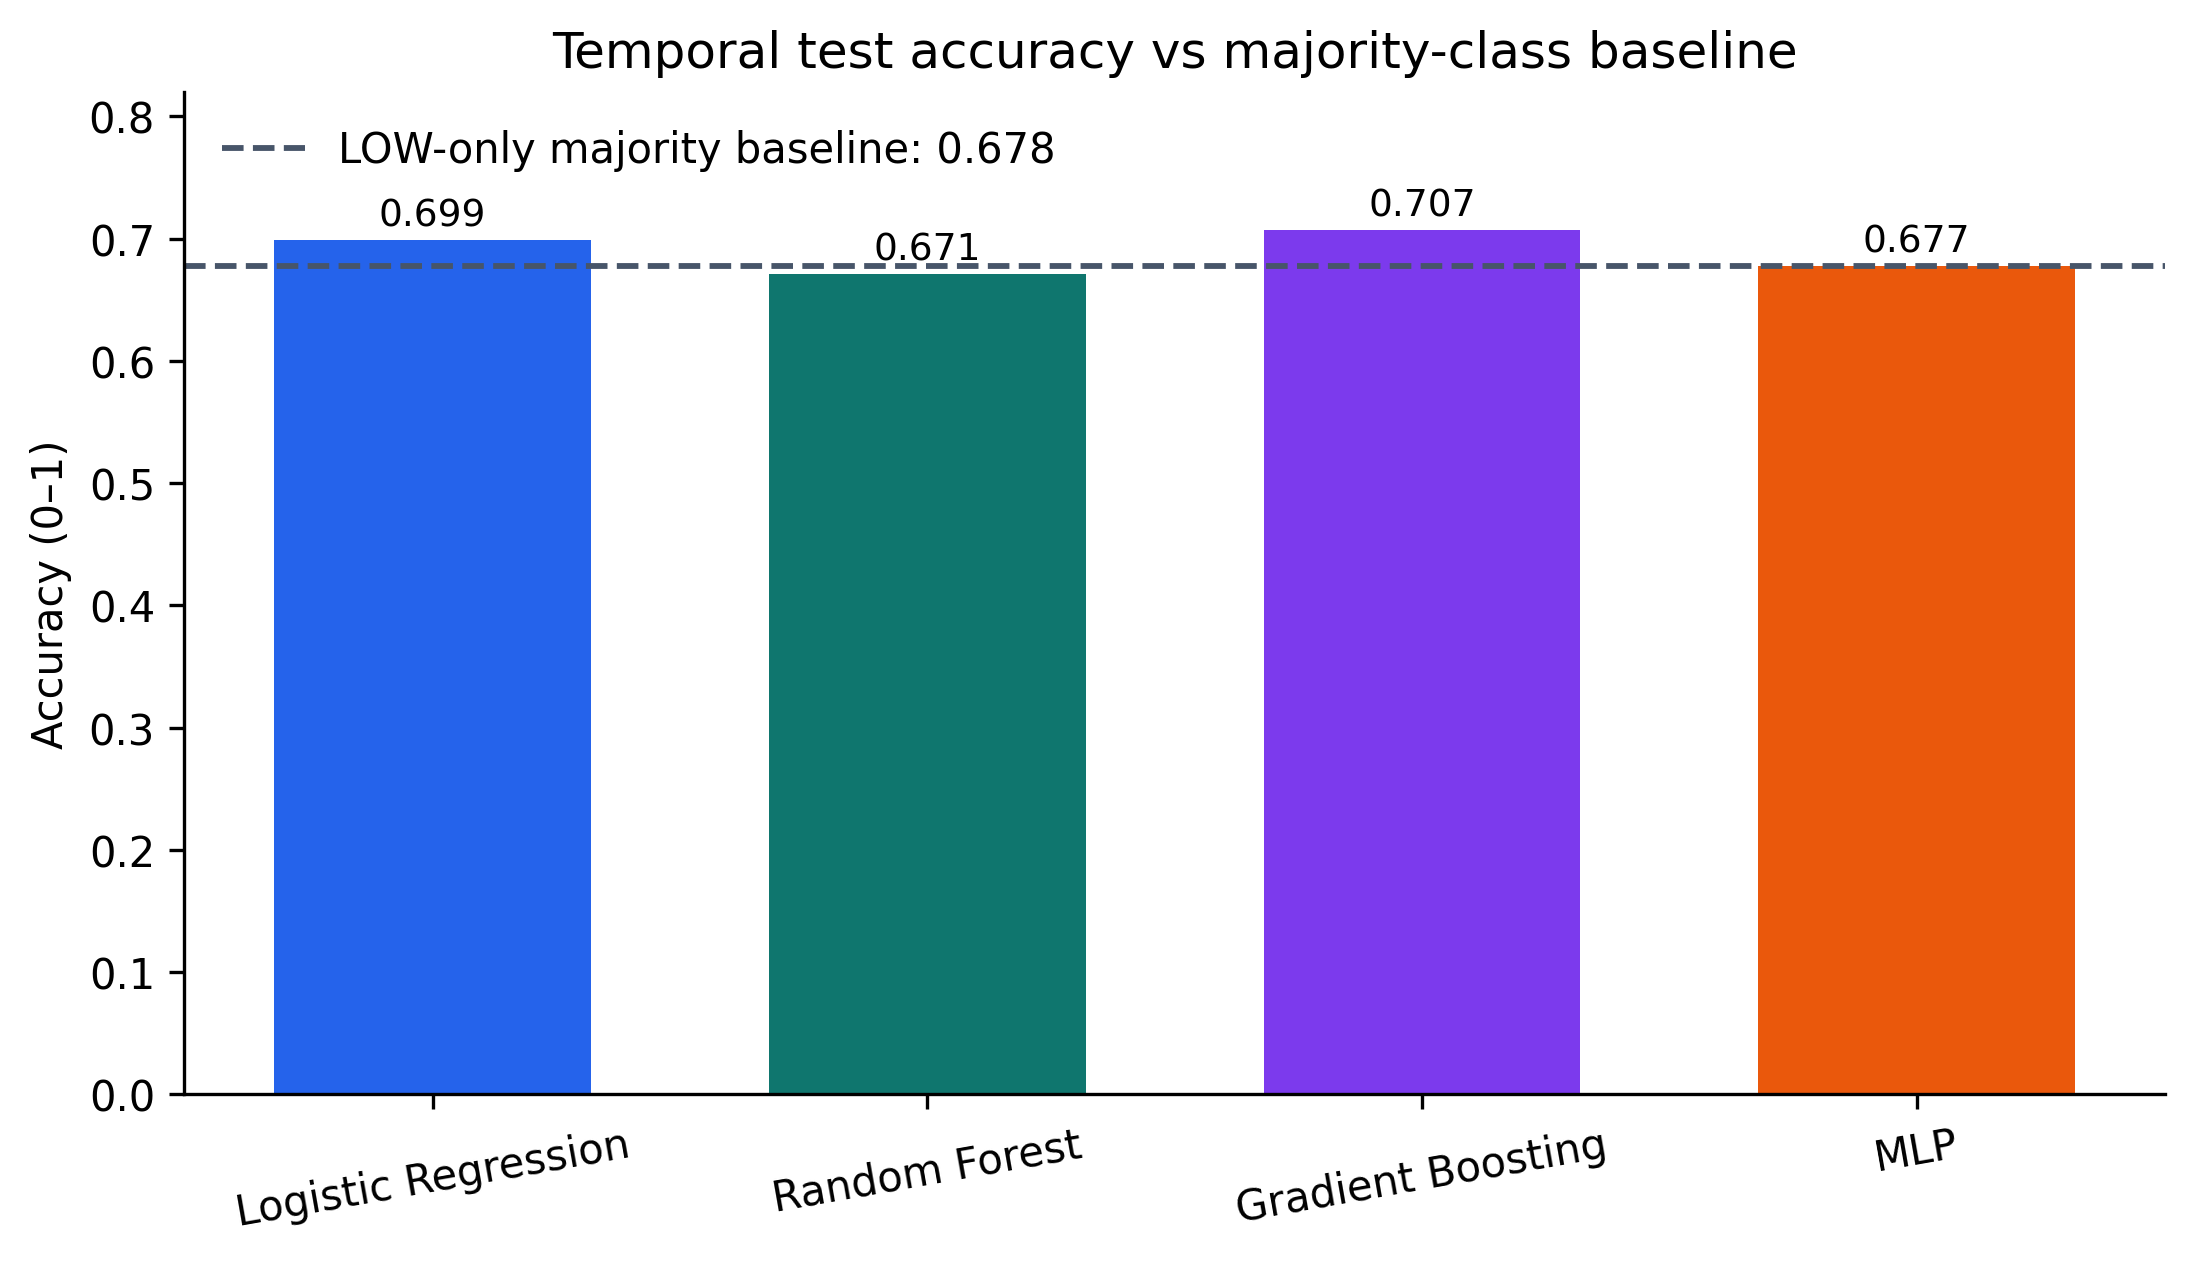
\includegraphics[width=.9\textwidth]{report_assets/graphs/model_vs_baseline.png}\caption{Test accuracy against the LOW-only majority baseline (0.678).}\label{fig:ml-baseline}\end{figure}
\begin{figure}[htbp]\centering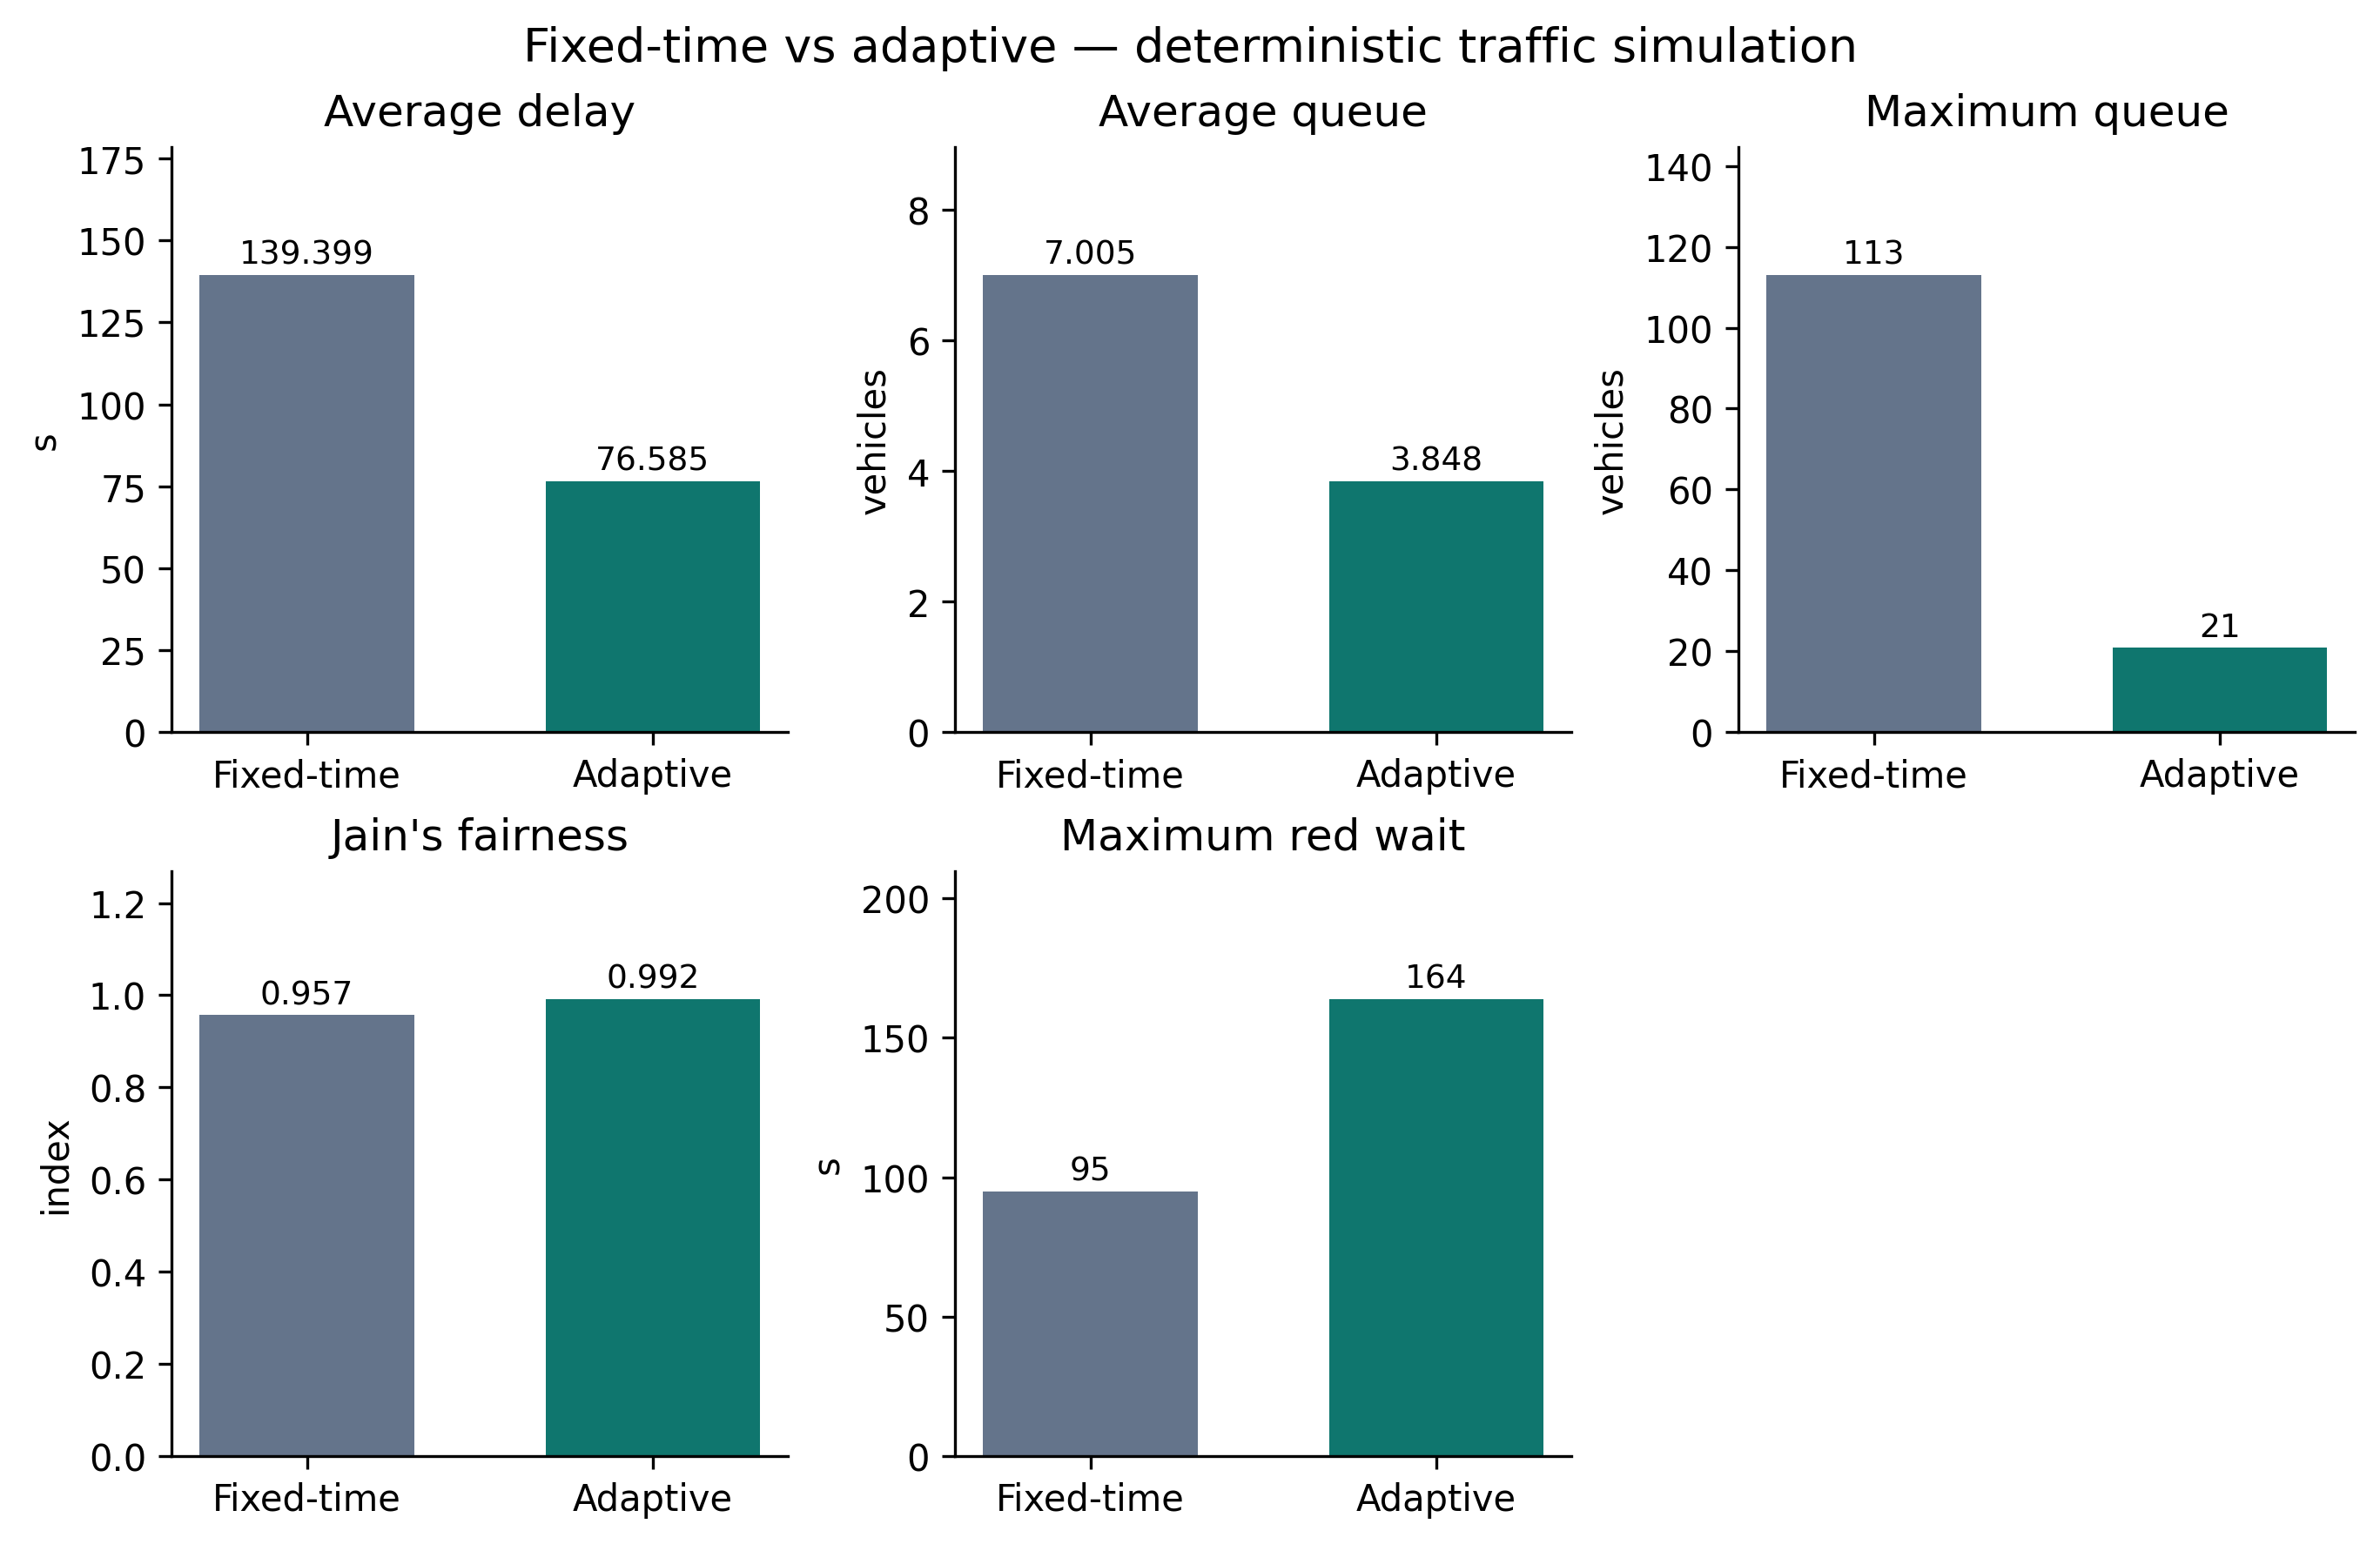
\includegraphics[width=.95\textwidth]{report_assets/graphs/fixed_vs_adaptive.png}\caption{Fixed-time versus adaptive results in deterministic simulation; average delay and queues improve while maximum red wait rises.}\label{fig:fixed-adaptive}\end{figure}
\begin{figure}[htbp]\centering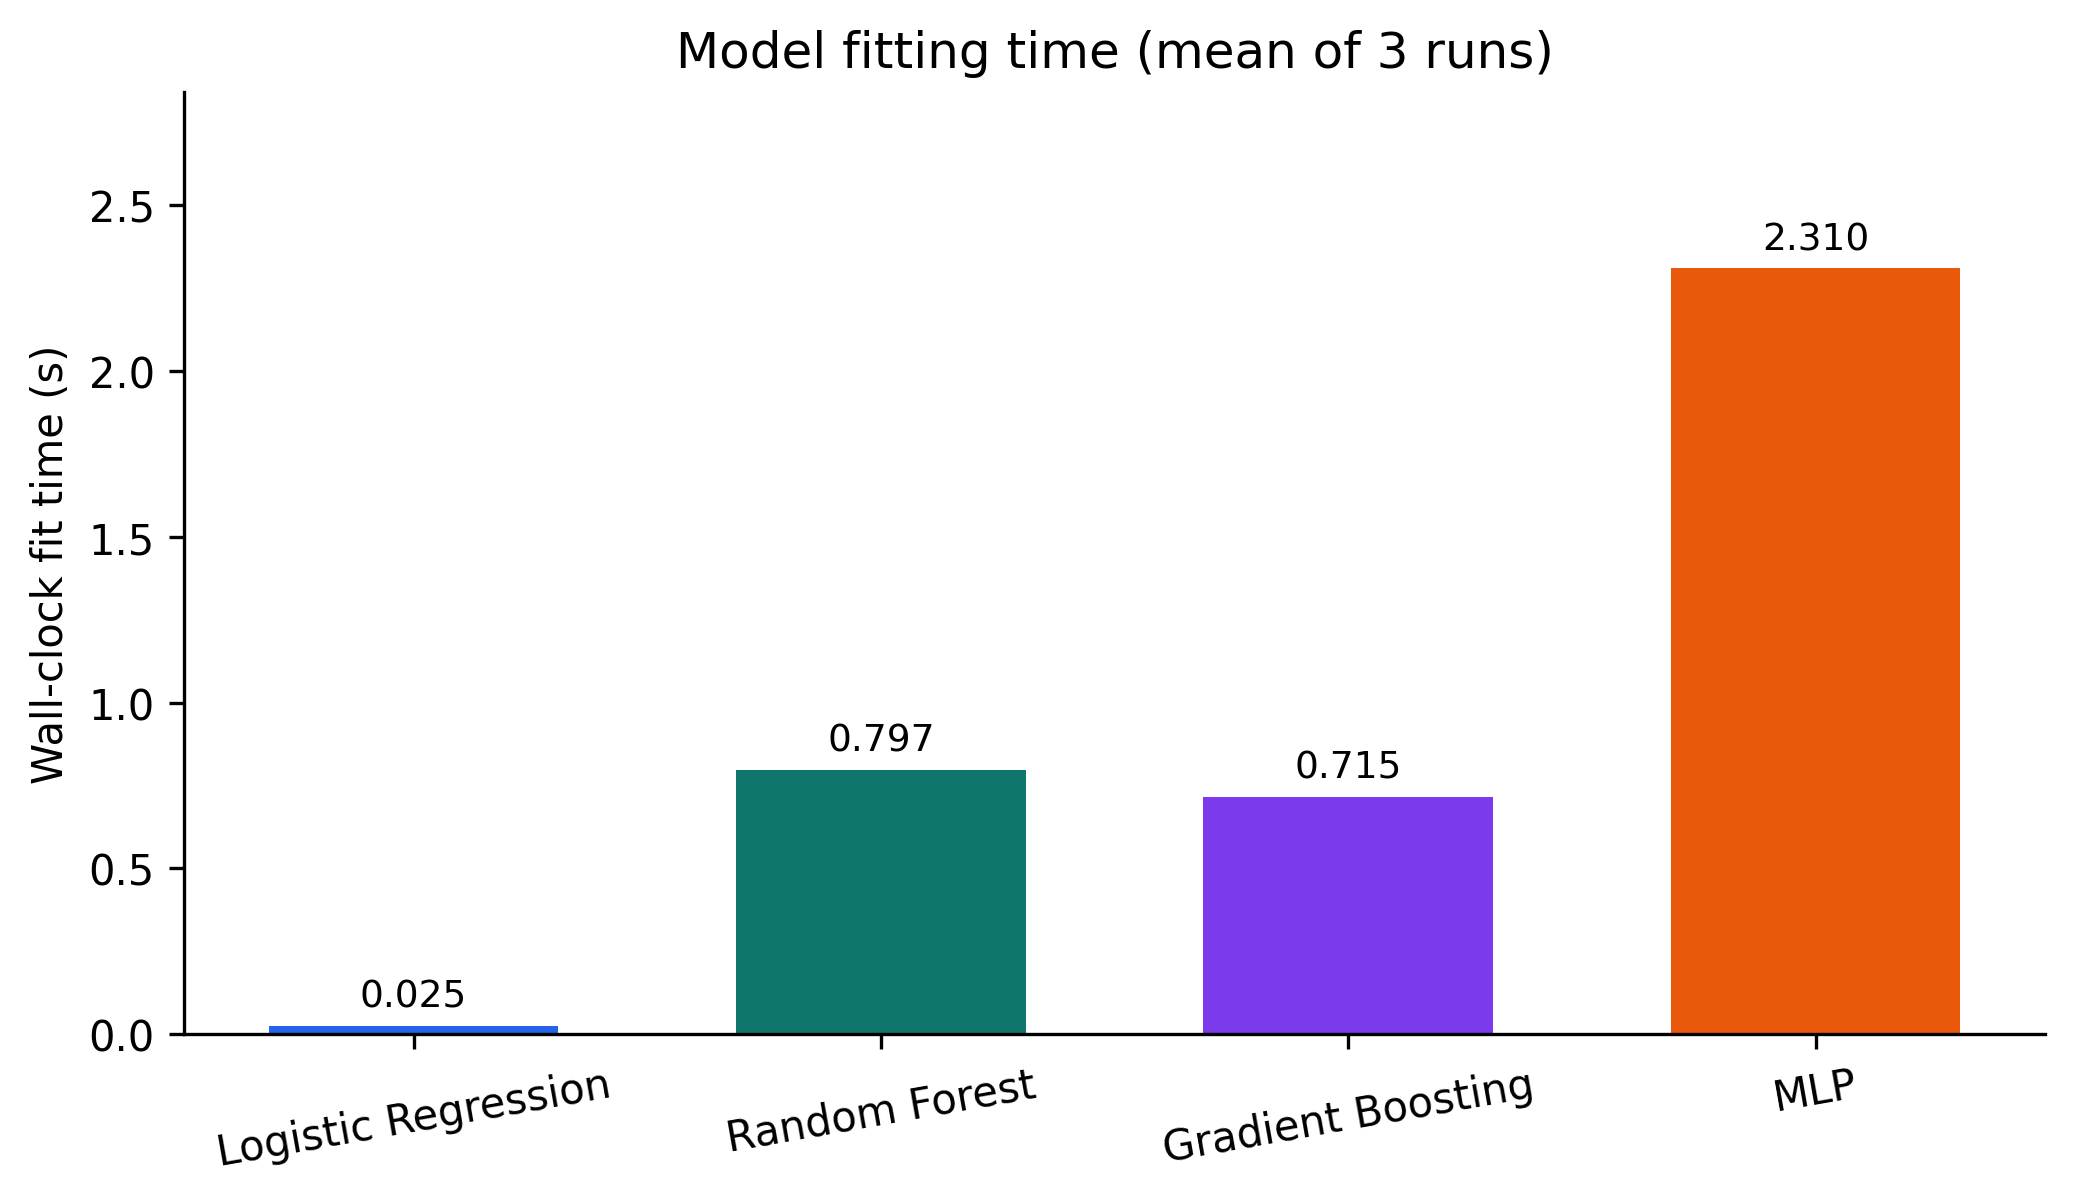
\includegraphics[width=.85\textwidth]{report_assets/graphs/benchmark_fit_time.png}\caption{Mean model fitting wall time over three benchmark runs.}\label{fig:benchmark-fit}\end{figure}
\begin{figure}[htbp]\centering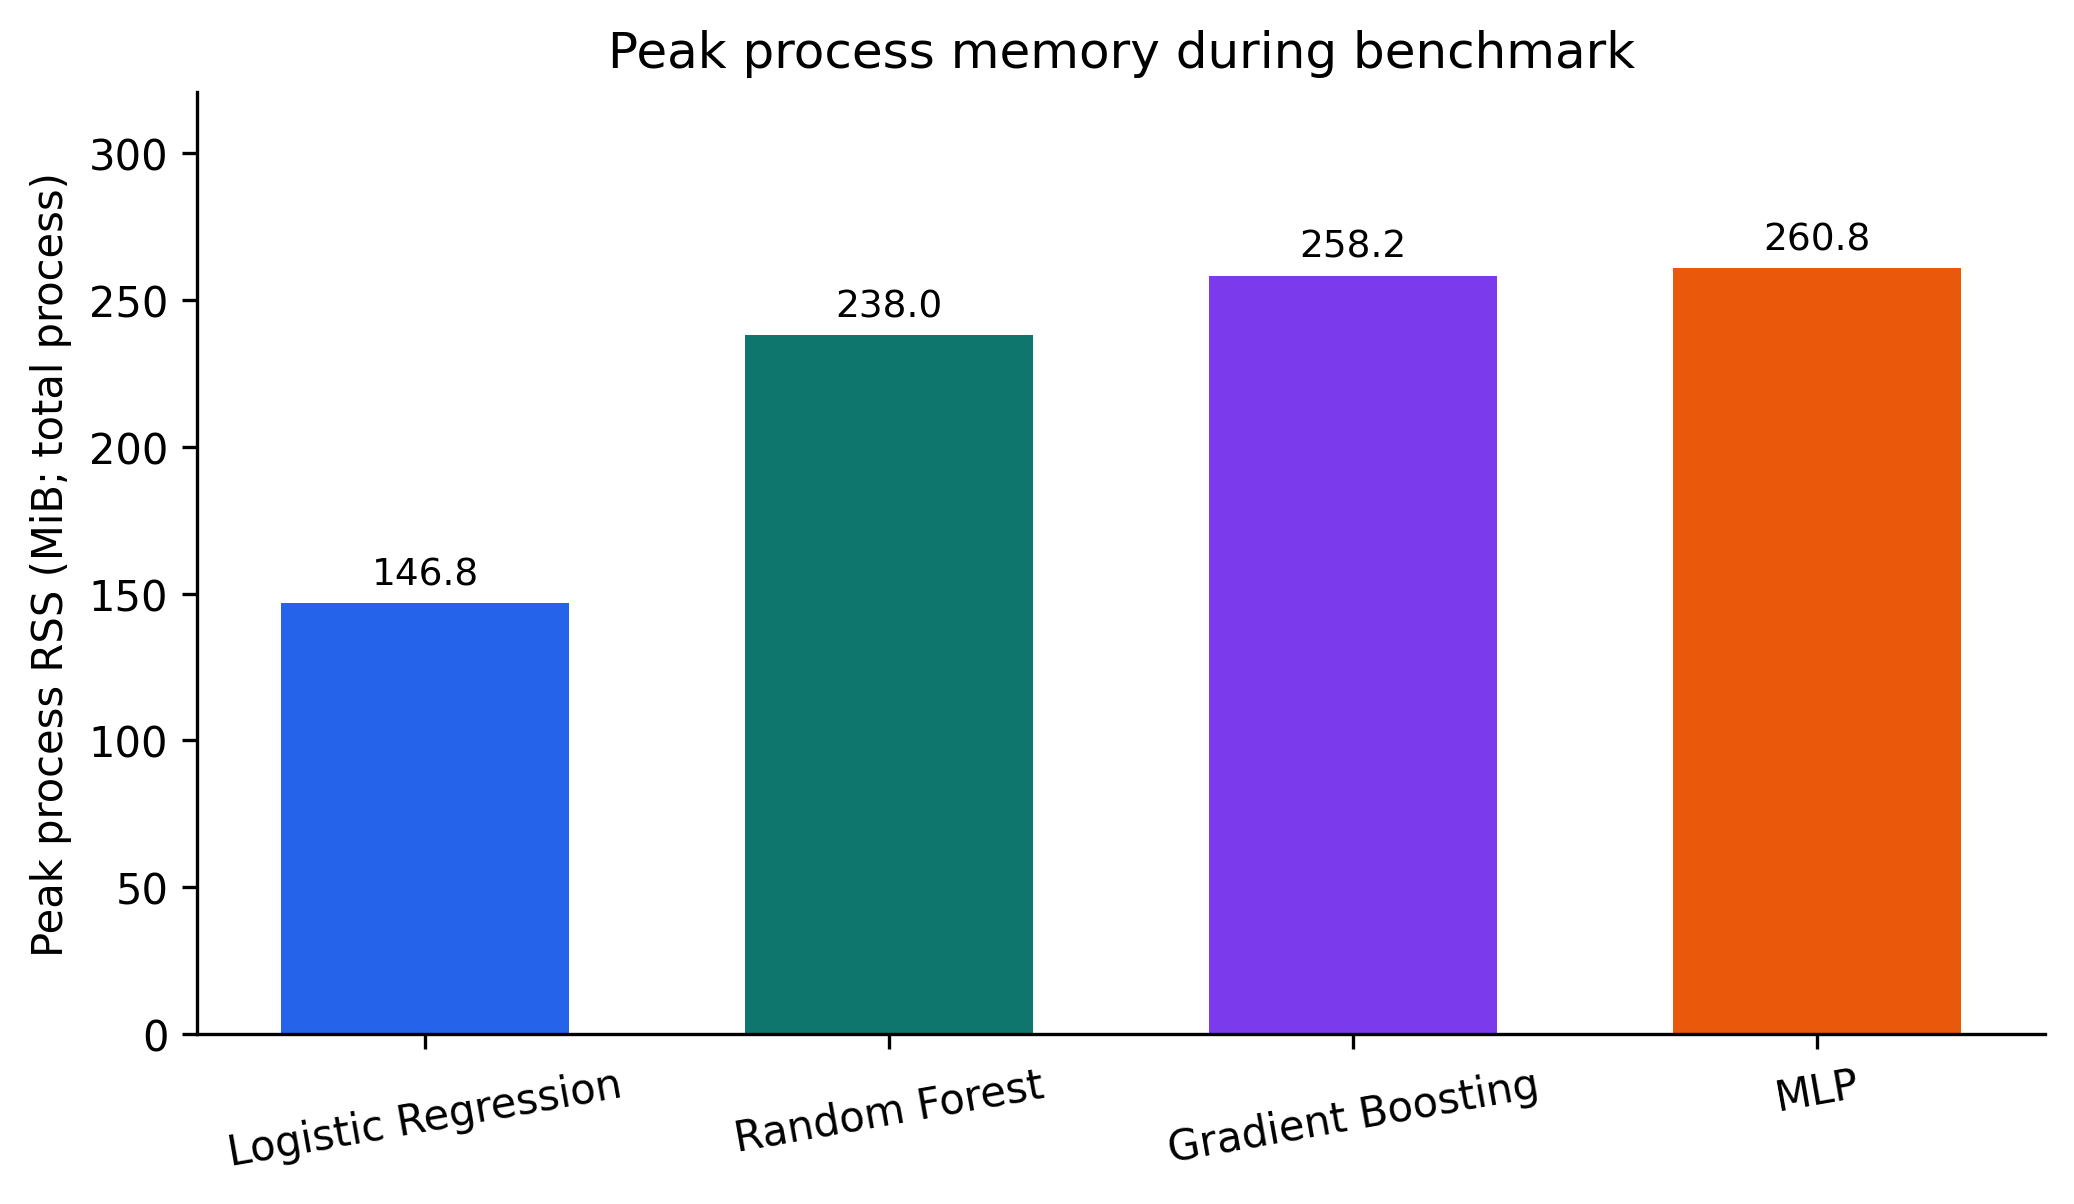
\includegraphics[width=.85\textwidth]{report_assets/graphs/benchmark_peak_rss.png}\caption{Peak process resident memory during benchmark (MiB).}\label{fig:benchmark-rss}\end{figure}
\begin{figure}[htbp]\centering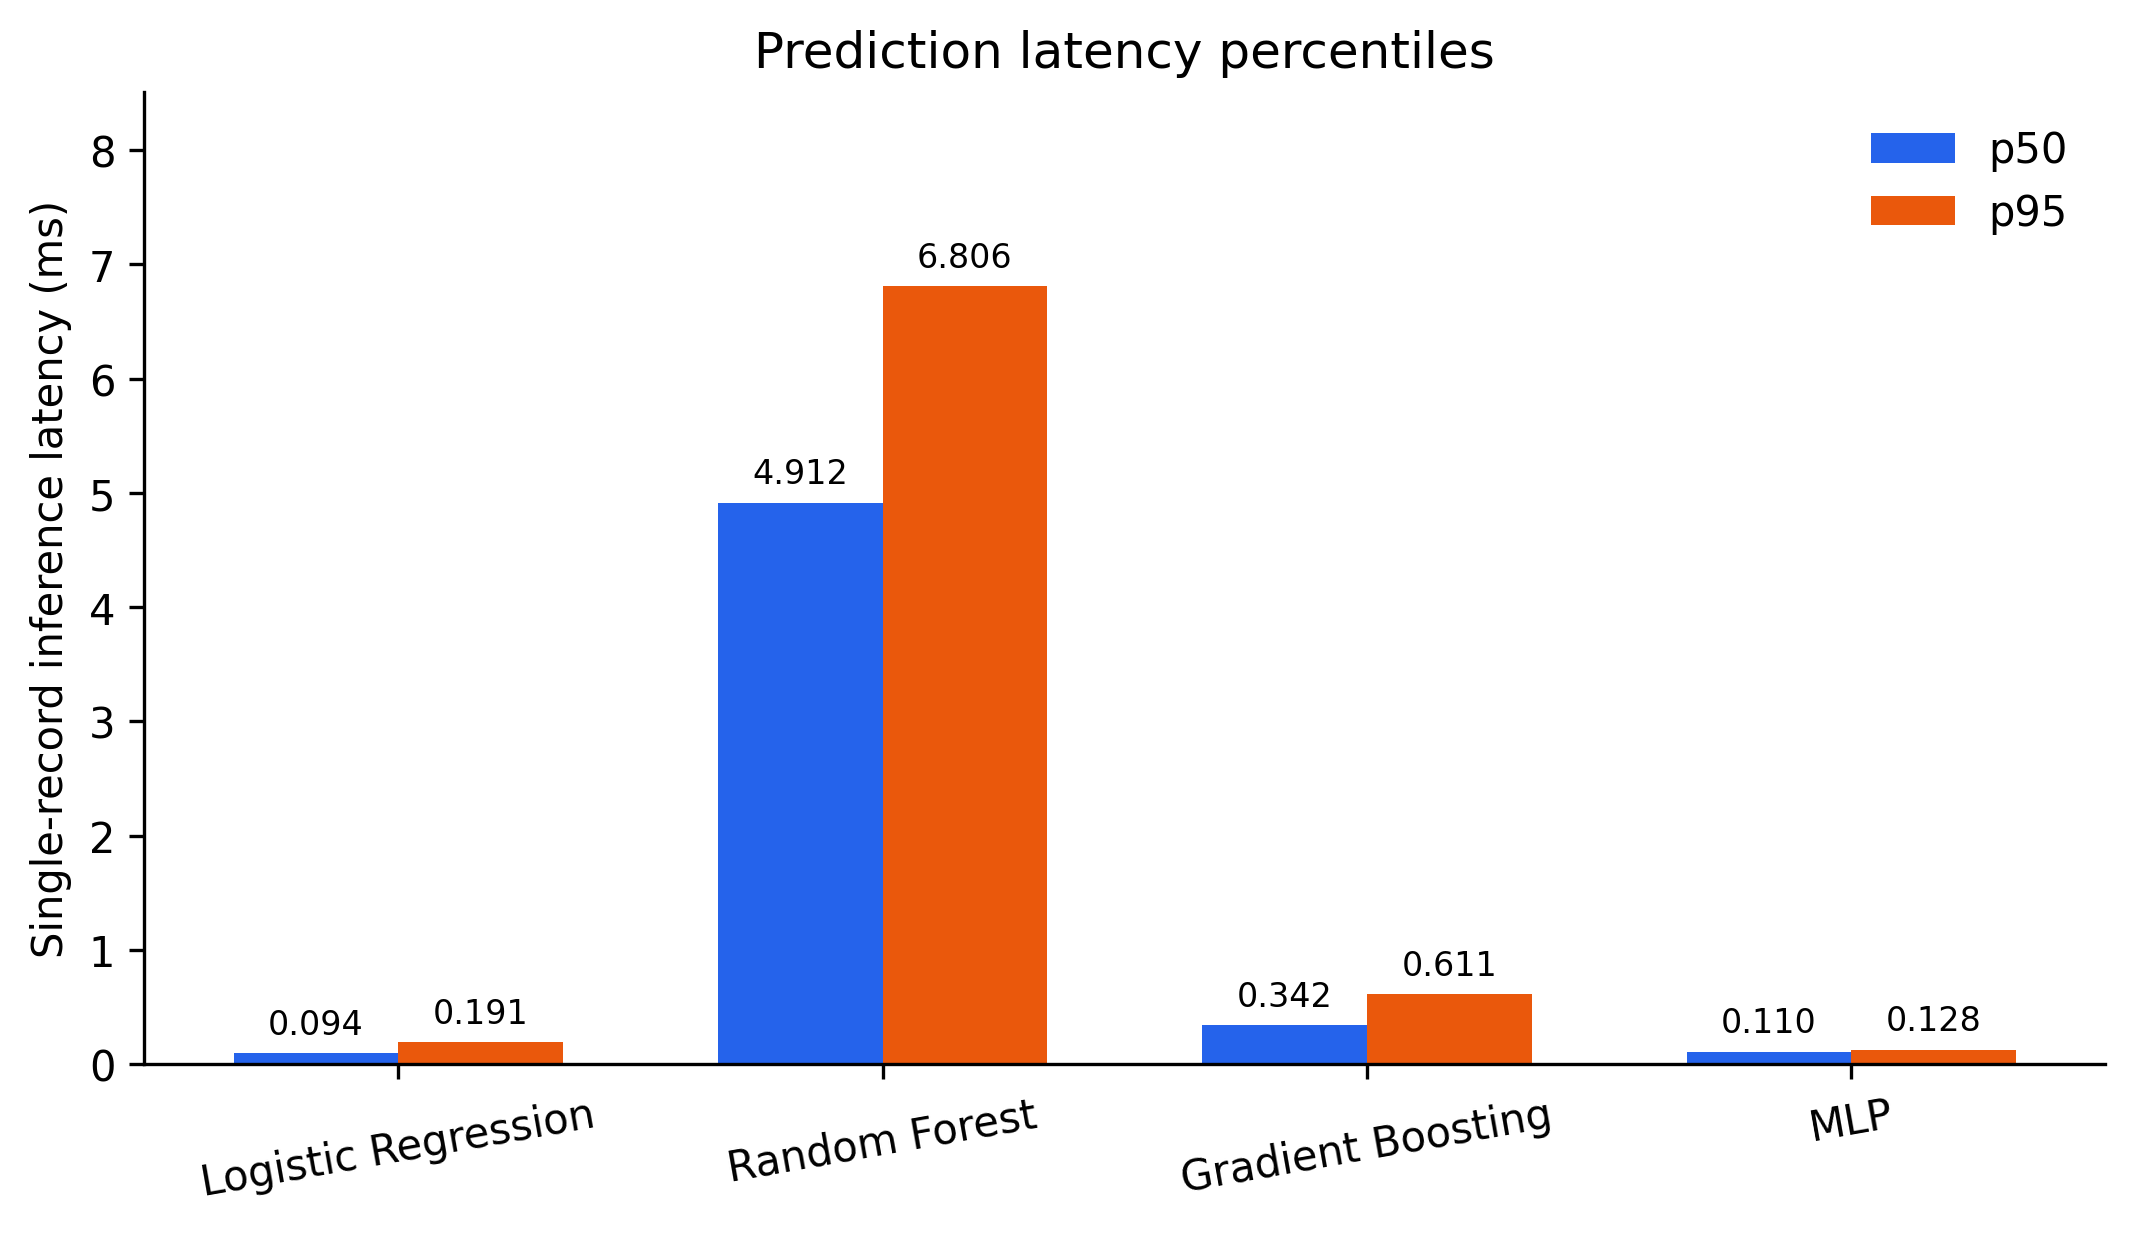
\includegraphics[width=.9\textwidth]{report_assets/graphs/benchmark_latency.png}\caption{p50 and p95 single-record prediction latency.}\label{fig:benchmark-latency}\end{figure}
\begin{figure}[htbp]\centering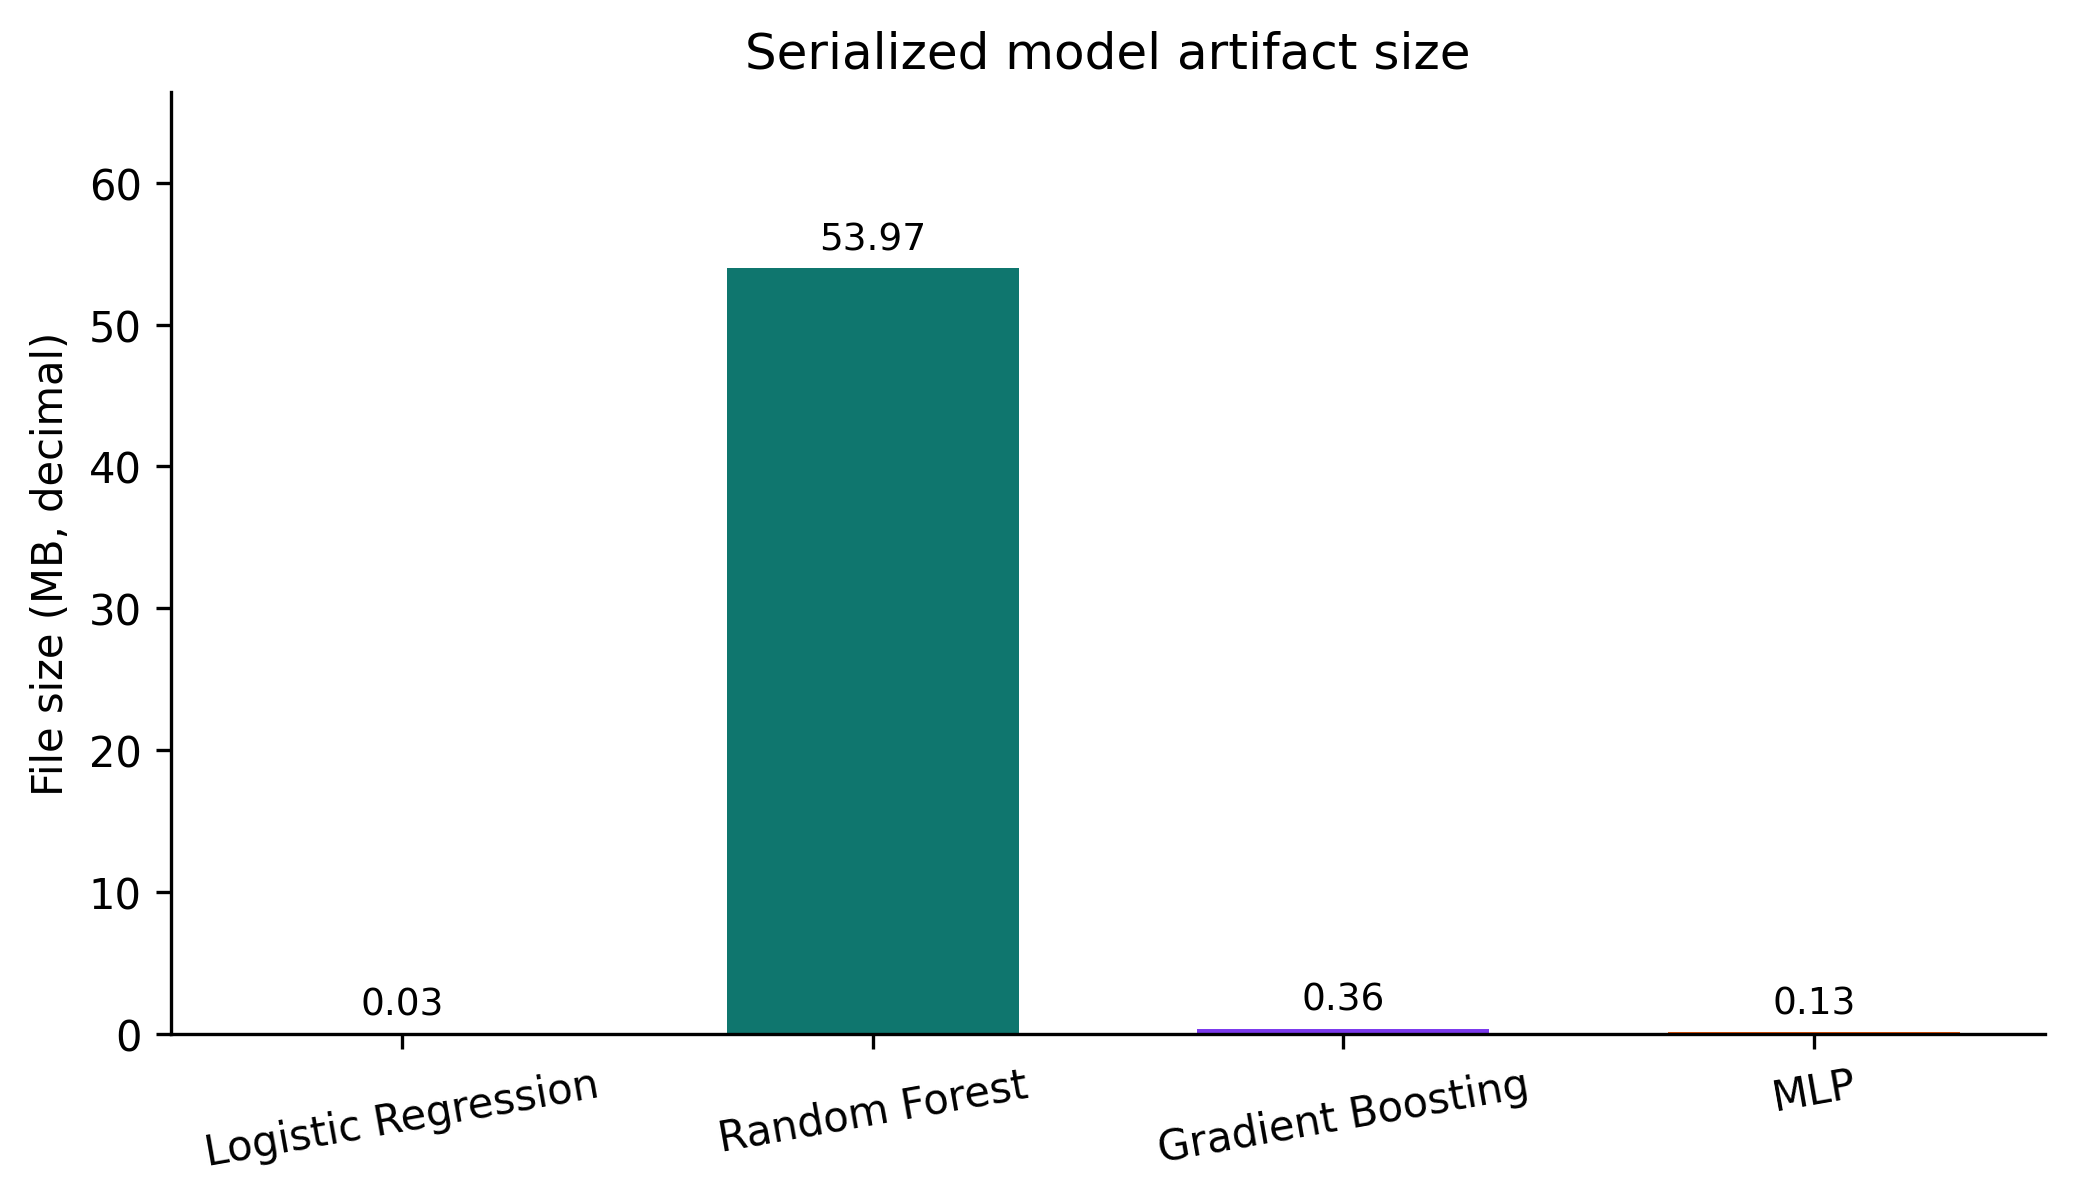
\includegraphics[width=.85\textwidth]{report_assets/graphs/benchmark_artifact_size.png}\caption{Serialized model artifact size (decimal MB).}\label{fig:benchmark-size}\end{figure}
